        %%******************************************%%
        %%                                          %%
        %%        Modello di tesi di laurea         %%
        %%            di Andrea Giraldin            %%
        %%                                          %%
        %%             2 novembre 2012              %%
        %%                                          %%
        %%******************************************%%

\begin{document}
    \frontmatter
    \begin{titlepage}
    \begin{center}
        \begin{LARGE}
            \textbf{\myUni}\\
        \end{LARGE}

        \vspace{10pt}

        \begin{Large}
            \textsc{\myDepartment}\\
        \end{Large}

        \vspace{10pt}

        \begin{large}
            \textsc{\myFaculty}\\
        \end{large}

        \vspace{30pt}
        \begin{figure}[htbp]
            \centering
            
\includegraphics[height=6cm]{unipd-logo}
        \end{figure}
        \vspace{30pt}

        \begin{LARGE}
            \textbf{\myTitle}\\
        \end{LARGE}

        \vspace{10pt}

        \begin{large}
            \textsl{\myDegree}\\
        \end{large}

        \vspace{40pt}

        \begin{large}
            \begin{flushleft}
                \textit{Relatrice}\\
                \vspace{5pt}
                \profTitle\ \myProf
            \end{flushleft}

            % You can tweak the spacing to have professor and student names on the same line
            % useful if the page is broken by a long thesis title and you need more space
            % \vspace{-52pt}

            \begin{flushright}
                \textit{Laureando}\\
                \vspace{5pt}
                \myName
            \end{flushright}
        \end{large}

        \vspace{40pt}

        \line(1, 0){338} \\
        \begin{normalsize}
            \textsc{Anno Accademico \myAA}
        \end{normalsize}
    \end{center}
\end{titlepage}

    \clearpage
\phantomsection
\thispagestyle{empty}

\hfill
\vfill

\noindent\myName: \textit{\myTitle,}
\myDegree,
\textcopyright\ \myTime.

    \cleardoublepage
\phantomsection
\thispagestyle{empty}
\pdfbookmark{Dedica}{Dedica}

\vspace*{3cm}

\begin{center}
    Lorem ipsum dolor sit amet, consectetuer adipiscing elit. \\ \medskip
    --- Oscar Wilde
\end{center}

\medskip

\begin{center}
    Dedicato a ...
\end{center}

    \cleardoublepage
\phantomsection
\pdfbookmark{Sommario}{Sommario}
\begingroup
\let\clearpage\relax
\let\cleardoublepage\relax
\let\cleardoublepage\relax

\chapter*{Sommario}

Il presente documento descrive il lavoro svolto durante il periodo di tirocinio formativo, della durata di circa trecentoventi ore complessive, dal laureando Gabriel Rovesti presso l'azienda Sync Lab, sede di Padova.
Durante il tirocinio era richiesto il raggiungimento di massima dei seguenti obiettivi.
\begin{itemize}
    \item studio autonomo delle tecnologie blockchain e dei protocolli di comunicazione;
    \item lo sviluppo di un'applicazione decentralizzata per comunicare e leggere dati da un contratto intelligente;
    \item l'implementazione di un'interfaccia grafica per la visualizzazione degli eventi registrati;
    \item l'integrazione del progetto con una libreria esterna per l'autenticazione usando le tecnologie \textit{Self Sovereign Identity} e \textit{Zero Knowledge Proof};
    \item la documentazione del lavoro svolto in un documento apposito dettagliante le tecnologie utilizzate, le scelte progettuali e le modalità di utilizzo del prodotto;
    \item l'utilizzo di \textit{React} per la parte frontend e \textit{Solidity} per la parte backend di comunicazione con la blockchain;
    \item l'utilizzo di \textit{TypeScript} per la parte di logica applicativa.
\end{itemize}

%In primo luogo era richiesto lo sviluppo di ...
%In secondo luogo era richiesta l'implementazione di un ...
%Tale framework permette di registrare gli eventi di un controllore programmabile, quali segnali applicati
%Terzo ed ultimo obbiettivo era l'integrazione ...

%\vfill

%\selectlanguage{english}
%\pdfbookmark{Abstract}{Abstract}
%\chapter*{Abstract}

%\selectlanguage{italian}

\endgroup

\vfill

    \cleardoublepage
\phantomsection
\pdfbookmark{Ringraziamenti}{ringraziamenti}

\begin{flushright}{
    \slshape
    ``Life is really simple, but we insist on making it complicated''} \\
    \medskip
    --- Confucius
\end{flushright}


\bigskip

\begingroup
\let\clearpage\relax
\let\cleardoublepage\relax
\let\cleardoublepage\relax

\chapter*{Ringraziamenti}

\noindent \textit{Innanzitutto, vorrei esprimere la mia gratitudine al Prof.\myProf, relatore della mia tesi, per l'aiuto e il sostegno fornitomi durante la stesura del lavoro.}

\noindent \textit{Desidero ringraziare con affetto i miei genitori per il sostegno, il grande aiuto e per essermi stati vicini in ogni momento durante gli anni di studio.}

\noindent \textit{Ho desiderio di ringraziare poi i miei amici per tutti i bellissimi anni passati insieme e le mille avventure vissute.}
\bigskip

\noindent\textit{\myLocation, \myTime}
\hfill \myName\endgroup

    \cleardoublepage
\pdfbookmark{\contentsname}{tableofcontents}
\setcounter{tocdepth}{4}
\tableofcontents
%\markboth{\contentsname}{\contentsname}
\clearpage

\begingroup
    \let\clearpage\relax
    \let\cleardoublepage\relax
    \let\cleardoublepage\relax

    % Figures list
    \phantomsection
    \pdfbookmark{\listfigurename}{lof}
    \listoffigures

    \vspace*{8ex}

    % Tables list
    \phantomsection
    \pdfbookmark{\listtablename}{lot}
    \listoftables

    \vspace*{8ex}
\endgroup

\cleardoublepage

    \cleardoublepage

    \mainmatter
    \chapter{Introduzione}\label{cap:introduzione}

\section{L'azienda e motivazioni della scelta}

Sync Lab è una \textit{software house} italiana nata a Napoli nel 2002 che, grazie ad una progressiva
maturazione delle sue competenze in ambito applicativo e tecnologico, è riuscita a diventare un
punto di riferimento per le aziende che intendono innovare i propri processi di business,
trasformandosi in un \textit{System Integrator}. L'azienda si è fatta notare sul mercato grazie alla proposta
di vari prodotti software, sviluppati all'interno del suo laboratorio di ricerca e sviluppo, 
conquistando importanti fette di mercato in ambito nazionale nei settori mobile, di sicurezza e videosorveglianza.
Ad oggi, Sync Lab conta più di 150 clienti e oltre 200 dipendenti disolcati nelle proprie sedi.
Queste sono situate a Napoli, Milano, Verona, Roma e Padova.
L'obiettivo principale dell'azienda è quello di fornire soluzioni tecnologiche innovative e di qualità
che possano soddisfare le esigenze dei propri clienti, garantendo un servizio di consulenza
e assistenza continuo e di alto livello.\\

Il mio contatto con l'azienda è avvenuto autonomamente, tramite l'invio di una candidatura spontanea
in base alle aziende presenti nella mappa di StageIt dell'anno 2022. Incuriosito dalle tematiche proposte e dai progetti presenti,
ho incontrato subito la massima disponibilità del mio attuale tutor, l'ingegner Fabio Pallaro, che mi ha fornito da suito un supporto valido
per la stesura del piano di lavoro e per la definizione degli obiettivi dello stage. Da parte sua e dell'azienda, vi è stata subito 
massima disponibilità e flessibilità nell'organizzazione del mio studio teorico e per la realizzazione del progetto,
dando una guida sulle possibili tecnologie e lasciandomi approfondire in autonomia le tematiche che più mi interessavano.

\begin{figure}[h]
    \centering
    
\includegraphics[width=0.4\textwidth, alt={Logo dell'azienda Sync Lab}]{immagini/synclab.png}
    \caption{Logo azienda Sync Lab}\label{fig:logo-synclab}
\end{figure}

\newpage

\section{Introduzione al progetto e idea dello stage}

Oggi più che mai è importante garantire la sicurezza dei propri dati e delle proprie informazioni, permettendo uno scambio sicuro
e protetto di dati sensibili tra due o più entità. Inoltre, è necessario garantire che le informazioni siano autentiche e non modificate,
per evitare che un utente malintenzionato possa alterare i dati e compromettere la sicurezza del sistema.
Sulla base di questa premessa, in accordo con l'azienda, si è deciso di sviluppare un progetto che permetta di esplorare 
le possibili applicazioni della tecnologia \gls{blockchaing} all'interno di un contesto reale e possibilmente applicabile in ambito aziendale. \\

In particolare, la piattaforma oggetto dello sviluppo durante il tirocinio ha come obiettivo principale il controllo dell'accesso ai contenuti
riservati, nel contesto dei film vietati ai minori. Grazie all'utilizzo della tecnologia \gls{blockchaing} e dello standard \gls{w3cg} \gls{ssig},
permettendo quindi di riconoscere i propri utenti evitando condivisione di informazioni, ma criptando i propri dati personali e verificando l'autenticità
dei dati trasmessi. Il progetto si pone quindi di risolvere il problema della condivisione di contenuti riservati, tramite l'utilizzo di tecnologie innovative
e la collaborazione con lo stagista ALessio De Biasi, utilizzando il codice di un progetto di un laureando magistrale presso Computer Science
dell'Università Ca' Foscari richiamato come libreria e di altri stagisti di laurea triennale con progetti similari basati sull'applicazione di tecnologie immutabili e decentralizzate. \\

Il suo utilizzo è molto simile ad altre piattaforme basate sulla condivisizione e fruizioni di contenuti multimediali:
l'utente si registra presso la piattaforma, fornendo i propri dati personali e la propria età. In questa fase, si ha il riconoscimento dell'utente
tramite l'utilizzo di un \gls{didg} e la creazione di un \gls{vcg} contenente i dati personali dell'utente, che verrà poi utilizzato per l'autenticazione
e la verifica dei dati. Una volta effettuata la registrazione, l'utente può accedere alla piattaforma e visualizzare i contenuti disponibili, permettendo l'accesso
anche a contenuti limitati qualora l'utente sia maggiorenne. Riconosciuta l'età dell'utente e verificata dalla piattaforma blockchain la sua autenticità,
l'utente può visualizzare il contenuto selezionato dimostrando tramite \gls{zkpg} di essere maggiorenne, senza dover fornire ulteriori informazioni personali. \\

Sulla base di queste premesse nasce il progetto \textbf{VerifiedMovies}.

\section{Way of Working e strumenti}
L'azienda Sync Lab adotta un modello di sviluppo \gls{agileg}, con l'obiettivo di monitorare e controllare lo sviluppo del progetto in modo flessibile e continuo, suddividendo le attività
in piccoli incrementi e con una collaborazione asincrona e distribuita. In particolare, il modello di sviluppo adottato è \gls{scrumg}, che prevede la suddivisione del progetto in sprint,
ovvero periodi di tempo di durata fissa, in cui vengono pianificate le attività da svolgere e i relativi obiettivi da raggiungere. Al termine di ogni sprint, viene effettuato su base settimanale
un incontro interno approfondito con il tutor aziendale, per discutere lo stato di avanzamento del progetto e le attività da svolgere per il successivo sprint. 
L'obiettivo del modello è dare maggiore importanza al ciclo di vita del \glslink{softwareg} e dei processi correlati, piuttosto che al prodotto finale, con l'obiettivo di migliorare la qualità del prodotto stesso.
Inoltre, grazie alla collaborazione con altri stagisti con progetti basati sugli stessi concetti e in generale con il team di sviluppo, è stato possibile condividere conoscenze e competenze,
discutere problemi e trovare soluzioni comuni, con un approccio incrementale e iterativo. \\

Gli strumenti utilizzati per lo sviluppo del progetto sono stati i seguenti:
\begin{itemize}
    \item{\textit{\textbf{Trello}}}, per la gestione delle attività e dei task da svolgere, condiviso con il tutor aziendale e verificato dallo stesso ad ogni incremento.
    All'interno di questo strumento è possibile monitorare le attività attraverso delle schede, simili a dei \textit{post-it}, differenziando le attività per specifiche colonne di avanzamento.
    Le diciture riportate dalle colonne sono generalmente come segue:
    \begin{itemize}
        \item{\textbf{Backlog}}: che contiene attività in corso di svolgimento, comprendenti schede con obiettivi di massima dello stage e delle sue singole parti e periodi;
        \item{\textbf{In corso}}, ossia attività in esecuzione e da realizzare entro la fine dello \textit{sprint};
        \item{\textbf{In verifica}}, ossia attività in attesa di verifica e considerate concluse, in attesa di essere spostate nella colonna \textit{Terminati} a seguito della \textit{sprint review};
        \item{\textbf{Terminati}}, cioè attività completate e verificate da parte del tutor aziendale.
    \end{itemize} 
    Un esempio di utilizzo di Trello è riportato in Figura \ref{fig:trello}.
    \begin{figure}[h]
        \centering
        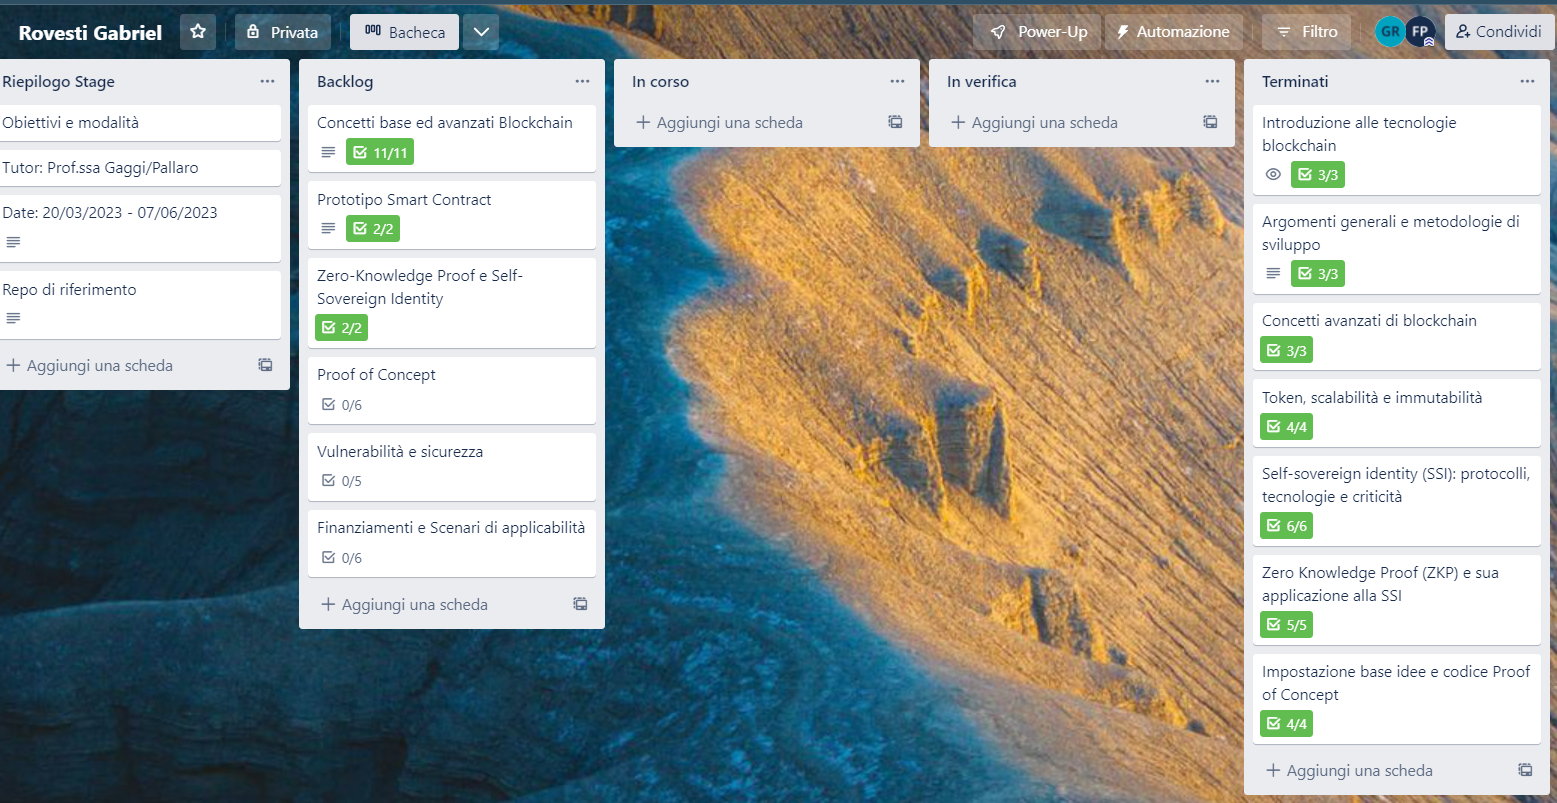
\includegraphics[width=1\textwidth, alt={Esempio di utilizzo di Trello}]{immagini/trello.png}
        \caption{Esempio di utilizzo di Trello}\label{fig:trello}
    \end{figure}

    \item{\textit{\textbf{Google Calendar}}}, per la pianificazione delle attività e degli incontri con il tutor aziendale, condiviso con il tutor stesso e con gli altri stagisti 
    e dipendenti di Sync Lab, capendo così e in anticipo le attività da svolgere e gli incontri da effettuare;
    
    \item{\textit{\textbf{Visual Studio Code}}}, \gls{ideg} utilizzato per la scrittura del codice sorgente e dei file di configurazione, con l'aggiunta di alcuni \textit{plugin} per la formattazione del codice e per la gestione dei file di configurazione 
    del progetto. All'interno di questo, è stato realizzato lo studio di esempi di codice e la realizzazione dell'intero progetto, con l'aggiunta di un sistema di \textit{linting} per la formattazione del codice e di un sistema di \textit{debugging} per il controllo del flusso di esecuzione del codice.
    Sempre tramite questo strumento, è stata scritto la tesi, attraverso l'utilizzo di un \textit{plugin} per la scrittura in \LaTeX;
    
    \item{\textit{\textbf{Diagrams.net}}}, per la realizzazione e la creazione delle immagini del documento, utilizzati per la documentazione e la strutturazione delle sezioni;
    
    \item{\textit{\textbf{StarUML}}}, per la realizzazione dei diagrammi \gls{umlg} del documento, quindi per i diagrammi dei casi d'uso e dei diagrammi delle classi;

    \item{\textit{\textbf{GitHub}}}, utilizzato internamente per la gestione del codice sorgente e dei file di configurazione, condiviso con il tutor aziendale e verificato dallo stesso ad ogni incremento.
    In particolare, è stato utilizzato il sistema di controllo versione \gls{gitg}, che permette di tenere traccia delle modifiche effettuate ai file e di gestire le varie versioni del codice e degli appunti interni 
    da me realizzati, per una migliore organizzazione e condivisione delle informazioni. Inoltre, è stato possibile condividere il codice sorgente con gli altri stagisti e dipendenti di Sync Lab,
    per garantire il versionamento e la condivisione delle modifiche effettuate.
    
    \item{\textit{\textbf{Discord}}}, social network utilizzato per la comunicazione interna tra i dipendenti di Sync Lab, 
    tramite la gestione di vari canali vocali e testuali divisi per argomento e per sedi interne aziendali. La suddivisione in gruppi e canali
    ha permesso di comunicare in modo efficace e veloce, condividendo informazioni e risorse utili per lo svolgimento del progetto, sia a livello di risorse 
    didattiche che per la risoluzione di eventuali dubbi e problemi. Inoltre, è stato possibile comunicare con gli altri stagisti in modo semplice e veloce,
    condividendo conoscenze e competenze e discutendo problemi e soluzioni comuni.
\end{itemize}

\section{Organizzazione del testo}

\subsection{Struttura del documento}

\begin{description}
    \item[{\hyperref[cap:tecnologie]{Il secondo capitolo}}] descrive le tecnologie studiate e utilizzate per lo sviluppo del progetto.
    
    \item[{\hyperref[cap:descrizione-stage]{Il terzo capitolo}}] approfondisce il percorso di tirocinio formativo, descrivendo precisamente gli obiettivi e le attività svolte durante il percorso,
    con relativa analisi dei rischi.
    
    %\item[{\hyperref[cap:analisi-requisiti]{Il quarto capitolo}}] approfondisce \ldots
    %
    %\item[{\hyperref[cap:progettazione-codifica]{Il quinto capitolo}}] approfondisce \ldots
    %
    %\item[{\hyperref[cap:verifica-validazione]{Il sesto capitolo}}] approfondisce \ldots
    %
    %\item[{\hyperref[cap:conclusioni]{Nel settimo capitolo}}] descrive \ldots
\end{description}

\subsection{Convenzioni tipografiche}
Riguardo la stesura del testo, relativamente al documento sono state adottate le seguenti convenzioni tipografiche:
\begin{itemize}
	\item gli acronimi, le abbreviazioni e i termini ambigui o di uso non comune menzionati vengono definiti nel glossario, situato alla fine del presente documento;
	\item per la prima occorrenza dei termini riportati nel glossario viene utilizzata la seguente nomenclatura: \emph{parola}\glsfirstoccur;
	\item i termini in lingua straniera o facenti parti del gergo tecnico sono evidenziati con il carattere \emph{corsivo}.
\end{itemize}


    \chapter{Tecnologie di interesse}\label{cap:tecnologie}

\intro{In questa sezione viene presentata una panoramica di base delle tecnologie oggetto del mio tirocinio, al fine
di descrivere in modo chiaro e conciso i concetti di base e le caratteristiche principali delle tecnologie utilizzate
nel progetto di stage e oggetto di studio autonomo e autodidatta.}

\section{Blockchain: concetti base}\label{sec:tecnologie-blockchain}

\subsection{Introduzione}\label{sec:tecnologie-blockchain-introduzione}

La \glsfirstoccur{\gls{blockchaing}} è una tecnologia che permette di memorizzare dati in maniera decentralizzata e distribuita.
Essa è una struttura dati che si comporta come un registro distribuito, salvando le informazioni in modo sicuro ed immutabile.
La struttura è stata introdotta nel 2008 da Satoshi Nakamoto, che ha pubblicato il suo white paper \textit{Bitcoin: A Peer-to-Peer Electronic Cash System}.
Nel 2009 è stato pubblicato il primo software open source per la blockchain, Bitcoin, che ha permesso di creare una moneta digitale decentralizzata. \\

A tal fine, non si devono confondere le cosiddette criptovalute con la blockchain. Di fatto, quest'ultima è solo la struttura che permette lo scambio di beni di qualsiasi tipo,
in modo sicuro, registrato ed immutabile. Una criptovaluta è invece una moneta digitale, che può essere scambiata con altre monete digitali o con beni fisici.
Essendo lo standard blockchain \textit{open source}, è possibile crearne di nuove con molta facilità.

Normalmente, viene utilizzata per memorizzare transazioni finanziarie, ma può essere utilizzata per memorizzare qualsiasi tipo di informazione.
Un altro suo nome è \textit{distributed ledger technology} (DLT), che indica che le sue informazioni sono registrate come su un libro mastro, in cui le singole componenti della rete,
definite nodi, possono accedere e modificare i dati, stabilendo se questi sono validi o meno. 

\subsection{Blocco}\label{sec:tecnologie-blockchain-blocco}

I dati delle blockchain sono strutturati in singoli blocchi, ciascuno contenente uno specifico set di informazioni.
Ogni blocco è collegato al precedente tramite un hash, che ne garantisce l'immutabilità.
I blocchi sono collegati in una catena, che viene aggiornata ogni volta che viene aggiunto un nuovo blocco.
Nello specifico, possiamo dettagliare una struttura formata dai seguenti (come descritto in figura \ref{fig:blocco}):
\begin{itemize}
    \item blocchi di dati;
    \item nonce, un numero generato casualmente alla creazione del blocco;
    \item l'hash del blocco precedente;
    \item il numero della transazione;
    \item \textit{timestamp} di generazione del blocco (data e ora).
\end{itemize} 

\begin{figure}[h]
    \centering
    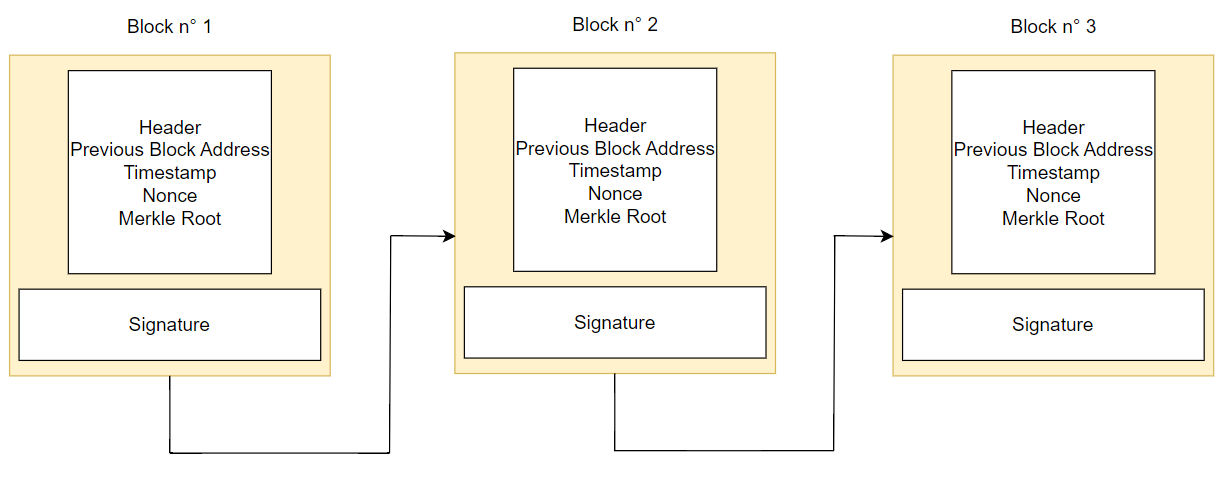
\includegraphics[width=0.6\textwidth, alt={Blocco all'interno di una blockchain}]{immagini/blocco.png}
    \caption{Blockchain vista come blocchi a catena} \label{fig:blocco}
\end{figure}

Per verificare l'integrità dei dati memorizzati, vengono usate delle strutture dati chiamati \textit{Merkle trees}, in cui ogni foglia rappresenta l'hash della transazione.
Le foglie vengono poi raggruppate in coppie, e l'hash di ogni coppia viene calcolato e memorizzato in un nodo superiore.
Il processo si ripete, fino a raggiungere la radice dell'albero, che rappresenta l'hash di tutte le transazioni contenute nel blocco.

\subsection{Transazione}\label{sec:tecnologie-blockchain-transazione}

Una transazione all'interno di una blockchain comporta il trasferimento di beni digitali, che possono essere valute, token, o qualsiasi altro tipo di informazione.
In questo senso, possiamo individuare vari componenti del processo di transazione:
\begin{itemize}
    \item{gli utenti}, che avviano le transazioni firmandole digitalmente con la propria chiave privata;
    \item{i \textit{miners}}, che attraverso un processo specifico definito come \textit{mining}, verificano la validità delle transazioni e le includono nel blocco successivo. 
    \item{i nodi}, che convalidano i blocchi di transazioni inviati dai miners prima che vengano aggiunti alle blockchain.
\end{itemize}

Nello specifico, possiamo descrivere una transazione in questo modo:
\begin{enumerate}
    \item l'utente avvia la transazione creando una firma digitale utilizzando la propria chiave privata. La firma dimostra che l'utente ha il diritto di inviare i beni;
    \item la transazione viene trasmessa alla rete di nodi o computer che eseguono il software della blockchain. Ogni nodo riceve la transazione e la aggiunge a un pool di transazioni non confermate;
    \item i nodi della rete convalidano la transazione per assicurarsi che il mittente abbia fondi sufficienti per completare la transazione e che questa sia conforme alle regole del protocollo blockchain;
    \item una volta che un numero sufficiente di nodi ha convalidato la transazione, questa viene aggiunta a un nuovo blocco di transazioni, insieme ad altre transazioni convalidate di recente;
    \item il blocco di transazioni viene aggiunto alla blockchain in un processo chiamato mining. L'estrazione comporta la risoluzione di complesse equazioni matematiche per creare un nuovo blocco, il che richiede una grande potenza di calcolo;
    \item una volta aggiunto il nuovo blocco alla blockchain, la transazione viene considerata confermata e i beni vengono trasferiti dall'indirizzo del mittente a quello del destinatario. La transazione è ora registrata in modo permanente sul libro mastro della blockchain, che può essere visualizzato e verificato da chiunque abbia accesso alla rete;
\end{enumerate}

\subsection{Wallet}\label{sec:tecnologie-blockchain-wallet}

Un \textit{wallet}, detto anche \textit{portafoglio}, è un software che permette di memorizzare e gestire le chiavi private e pubbliche, e di inviare e ricevere transazioni.
In particolare, possiamo più propriamente definirli portachiavi, in quanto non contengono realmente i beni digitali, ma le chiavi utilizzate per accedervi.
L'utente dispone in ogni momento di:
\begin{itemize}
    \item una chiave pubblica, usata per inviare messaggi e ricevere pagamenti. È un codice univoco che identifica l'utente;
    \item una chiave privata, usata per firmare i messaggi e per accedere ai propri beni digitali. È un codice segreto che deve essere conservato in modo sicuro.
\end{itemize} 

Ogni wallet dispone di una frase segreta, che contiene tutte le informazioni necessarie per recuperare ed accedere ai fondi del proprio portachiavi.

Inoltre, dispone di un proprio indirizzo, matematicamente derivato dalla stessa chiave pubblica mediante l'operazione di \textit{hashing}, con una lunghezza di 160 bit.
Ciascuno è \textit{pseudonimo}, in quanto non appartiene nello specifico ad una persona, ma non è completamente anonimo. \\
È importante tenere la chiave privata in un luogo sicuro e non condividerla con nessuno, in quanto è l'unica cosa che garantisce l'accesso ai propri fondi.
Distinguiamo due tipi di wallet:
\begin{itemize}
    \item \textit{hot wallet}, che sono i portafogli online, dunque più vulnerabili al rischio di \textit{hacking};
    \item \textit{cold wallet}, che sono i portafogli offline, quindi considerati più sicuri, in quanto si collegano ad Internet principalmente per effettuare le transazioni.
\end{itemize}

\subsection{Mining}\label{sec:tecnologie-blockchain-mining}

Il processo di \textit{mining} consente di creare nuovi blocchi sulla catena, al fine di convalidare le transazioni e ottenere nuove criptovalute come ricompensa per il proprio `sforzo'.
Questo obiettivo viene raggiunto attraverso un processo chiamato \textit{consenso}, che prevede la risoluzione di complessi puzzle matematici utilizzando la potenza di calcolo.
Il miner che riesce a risolvere il puzzle prima degli altri, vince il diritto di aggiungere il blocco alla blockchain. \\

Questo processo è composto da due fasi:
\begin{itemize}
    \item \textit{hashing}, che consiste nella risoluzione di un puzzle matematico, che consiste nel trovare un numero che, una volta applicata una funzione di hash, abbia un valore inferiore ad un valore prefissato. Il valore di questo numero viene chiamato \textit{nonce};
    \item \textit{ricerca del consenso}, che consiste nella verifica della validità del blocco, che viene effettuata da tutti i nodi della rete. Se il blocco è valido, viene aggiunto alla blockchain.
\end{itemize}

I minatori (miners) utilizzano un software speciale per risolvere il problema matematico incredibilmente complesso 
di trovare un nonce che generi un hash accettato. Poiché il nonce è di soli 32 bit e l'hash di 256, ci sono circa quattro miliardi 
di possibili combinazioni nonce-hash che devono essere estratte prima di trovare quella giusta. \\

Quando un blocco viene estratto con successo, la modifica viene accettata da tutti i nodi della rete e il miner viene ricompensato finanziariamente. 
Il primo minatore che risolve il puzzle e aggiunge un nuovo blocco alla blockchain viene ricompensato con un blocco di criptovaluta di nuovo conio.
Il processo richiede un software specializzato e una grande potenza di calcolo, che può essere ottenuta utilizzando un computer o un gruppo di computer con grosso dispendio di energia e risorse.

\subsection{Algoritmi di consenso}\label{sec:tecnologie-blockchain-algoritmi}
Il meccanismo di ricerca di consenso prevede numerose varianti, che differiscono per il modo in cui i nodi della rete si accordano per aggiungere un nuovo blocco alla blockchain.\\
Possiamo principalmente distinguere:
\begin{enumerate}
    \item\textit{{Proof of Work (PoW)}}, basato nella ricerca di un hash (una stringa di numeri e lettere) che soddisfa una determinata condizione, detta target. La condizione target richiede 
    che l'hash del nuovo blocco sia inferiore a un determinato valore. Questo valore viene stabilito in base alla difficoltà della blockchain, che viene regolata automaticamente per mantenere 
    il tempo medio di creazione di un nuovo blocco costante. Questo processo è descritto visivamente dalla figura \ref{fig:pow}.

    Il primo miner che trova correttamente l'hash del blocco viene ricompensato in criptovaluta per il lavoro svolto.
    Questo meccanismo garantisce sicurezza nella rete, perché rende difficile ad un attaccante malintenzionato
    compromettere la sicurezza della rete non avendo la stessa potenza di calcolo.
    
    Questa è attualmente utilizzata in \textit{Bitcoin}, in cui il tempo medio della formazione di blocchi è di 10 minuti circa, oppure la piattaforma \textit{Ethereum}, altro importante esempio di blockchain.
    Si consideri che ne esistono varie tipologie, in cui ciascuna cerca di ridurre il consumo energetico dando prova del lavoro svolto (\textit{Meaningful}) oppure assicurandosi che
    i nodi abbiano calcolato correttamente dopo un certo tempo (\textit{Delayed}).
    Il principale svantaggio del PoW è che richiede un elevato consumo energetico, che può essere risolto con l'utilizzo di algoritmi di consenso alternativi.

    \begin{figure}[h]
        \centering
        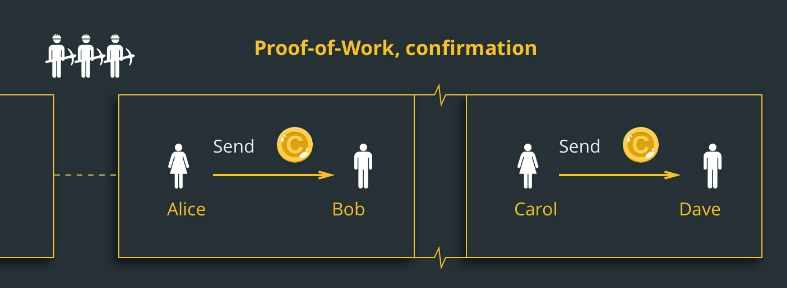
\includegraphics[width=0.6\textwidth, alt={Come avviene il processo di conferma in Proof of Work}]{immagini/proof-of-work.png}
        \caption{Processo di conferma in Proof of Work}\label{fig:pow}
    \end{figure}

    \item\textit{{Proof of Stake (PoS)}}, che si si basa sulla detenzione di una certa quantità di criptovaluta come garanzia per la validazione delle transazioni. 
    L'alto consumo di energia dell'algoritmo precedente ha portato ad algoritmi come il \textit{Proof of Stake}, i nodi della rete bloccano una certa quantità di criptovaluta come `punteggio'
    per dimostrare che hanno un interesse nella corretta validazione delle transazioni. 
    Questo punteggio viene utilizzato come base per la selezione del nodo che convalida la transazione successiva. 
    
    A differenza del PoW, non ci sono miner coinvolti nel processo. Al loro posto, i partecipanti alla rete che 
    vogliono essere coinvolti nella verifica della validità delle transazioni e nella creazione di blocchi nella rete 
    devono detenere una certa quota nella rete, per esempio mettendo una certa quantità di moneta della rete in un portafoglio collegato 
    alla sua blockchain. Questo processo è noto come `placing a stake' o `staking', che può essere tradotto come il fatto di mettere i propri interessi in gioco. 
    
    Pertanto, le reti PoS sono basate su algoritmi deterministici, il che significa che i validatori dei blocchi sono eletti a seconda della natura della posta in gioco. 
    Pur risultando meno intensiva in termini di energia rispetto alla PoW, il sistema risulta essere sbilanciato a favore dei produttori di blocchi oppure a favore degli utenti ricchi, 
    poiché i validatori con più moneta hanno più possibilità di essere eletti. 
    Alcune varianti di questo algoritmo prevedono infatti di scegliere dei nodi delegati per convalidare le transazioni e avere più controllo (\textit{Delegated}), 
    oppure di scegliere i validatori in base alla quantità di moneta che hanno investito (\textit{Proof of Burn}).

\end{enumerate}

\subsection{Tipi}\label{sec:tecnologie-blockchain-tipi}
Una prima categorizzazione delle blockchain avviene distinguendole in base ai permessi. Nello specifico:
\begin{itemize}
    \item \textit{permissioned}, in cui i nodi della rete sono controllati da un ente centrale, che può essere un'azienda, un'organizzazione o un'istituzione.
    Esse limitano l'accesso alla rete a determinati nodi e possono anche limitare i diritti di tali nodi su tale rete. Le identità degli utenti di una blockchain autorizzata sono note agli altri utenti della blockchain autorizzata.
    Queste sono spesso utilizzate da aziende per la gestione di dati sensibili o convalida di transazioni;
    \item \textit{permissionless}, che non richiedono alcun permesso per partecipare e permettono agli utenti di essere pseudoanonimi 
    (usando uno pseudonimo non si rivela alcun dettaglio relativo all'identità personale) e non restringono i permessi dei nodi. Queste ultime tendono ad essere più sicure delle precedenti, avendo vari nodi che convalidano le singole transazioni.
    Di fatto, sono usate dalle varie blockchain, come ad esempio quella di Bitcoin.
\end{itemize}

Fatta tale premessa, possiamo distinguere:
\begin{itemize}
    \item \textit{public}, in cui chiunque abbia accesso alla rete può partecipare e diventare un nodo autorizzato nella blockchain. Di fatto sono sicure, ma non anonime e molto meno scalabili.
    Una loro futura implementazione sarà all'interno dei sistemi di votazioni elettroniche.
    \item \textit{private}, in cui i singoli nodi sono controllati da un ente centrale, che opera in una rete chiusa e, come tali, restringono la natura di blockchain, dato che richiede controllo centralizzato dei singoli nodi per poter funzionare.
    Queste sono utilizzate da parte di alcune banche per la gestione dei loro sistemi di pagamento.
    \item \textit{hybrid}, in cui alcuni nodi sono pubblici e altri sono privati, normalmente utilizzata per eseguire convalide delle transazioni presenti al suo interno.
    Microsoft utilizza una blockchain di identità digitale basata sul meccanismo ibrido.
    \item \textit{consortium}, all'interno della quale i nodi sono controllati da un ente centrale, ma la rete è aperta a tutti i membri del consorzio, portando anche qui ad una privatizzazione e centralizzazione della rete.
    IBM sta utilizzando una piattaforma basata sulla gestione dei pagamenti per banche ed aziende partner.
\end{itemize}

\section{Blockchain: concetti avanzati}\label{sec:tecnologie-blockchain-avanzate}

\subsection{Token}\label{sec:tecnologie-blockchain-avanzate-token}
Possiamo definire i token come unità di valore accettate da una comunità e costruite su una blockchain pre-esistente (dunque, non possono essere minati).
Possono essere usati per rappresentare asset fisici come l'oro o l'immobiliare, oppure per rappresentare beni digitali 
come i dati o i diritti di accesso a servizi. Essendo registrati su una blockchain, sono immutabili e possono essere trasferiti in modo sicuro e trasparente da un proprietario all'altro. \\

Per utilizzare i token, gli utenti devono prima avere un portafoglio digitale, ovvero un'interfaccia che consente loro 
di accedere alla blockchain e interagire con essa. Una volta che un utente ha un portafoglio, 
può ricevere e inviare token. Per ricevere i token, l'utente deve fornire il proprio indirizzo del portafoglio al mittente, 
che poi invia i token all'indirizzo fornito. Per inviare i token, l'utente deve avere abbastanza token nel proprio portafoglio e deve conoscere l'indirizzo del destinatario a cui inviare i token. \\

Ogni bene viene considerato \textit{asset}, in quanto non riproducibile e non falsificabile, esistente solo in forma digitale e quindi non fisica. 
Un token può essere lanciato sul mercato tramite un \textit{initial coin offering} (ICO),
che è un'offerta pubblica iniziale di token, al fine di finanziare nuovi progetti e comprenderne il nuovo valore.
\\ 
Come per le blockchain, gli asset non sono regolamentati da un organo centrale, pertanto è possibile raccogliere fondi senza nuovi intermediari e così creare
nuovi progetti, adeguatamente documentati tramite un \textit{white paper} che descrive il progetto e il suo funzionamento. 
Il loro processo di creazione dei token nelle blockchain viene definito come \textit{minting}, in cui un creatore mette a disposizione un certo numero di token,
che possono essere acquistati dai partecipanti. \\

Principalmente, i token possono essere classificati in base al loro scopo:
\begin{itemize}
    \item \textit{Utility token}, che consentono di acquistare un determinato bene o servizio e conferisce al titolare un diritto di opzione per l'acquisto o somministrazione di cose o per la fornitura di servizi (attuali o futuri). 
    \item \textit{Security token}, che sono token che rappresentano un diritto di proprietà su un bene fisico o digitale.
    \item \textit{Payment token}, più comunemente noti come `crypto'. Come si può intuire, questi token sono utilizzati per acquistare e vendere beni e pagare le commissioni delle transazioni basate sulla blockchain senza la necessità di un intermediario.
\end{itemize}

I token, principalmente, sono caratterizzati dal fatto di essere spendibili e scambiabili con altri beni dal valore equivalente, ossia `fungibili'.
In questo senso, è possibile citare:
\begin{itemize}
    \item \textit{token fungibili (fungible tokens)}, che hanno la caratteristica di essere non uniche, divisibili e avere un chiaro valore di mercato, quindi scambiabili sempre con altri beni dello stesso valore;
    \item \textit{token non fungibili (non fungible tokens  NFT)}, beni fisici o digitali unici ed irripetibili. Questi vengono definiti come tali in quanto non possono essere scambiati con altri beni dello stesso valore,
    e per natura delle stesse blockchain, sono considerati immutabili. Infatti, l'utente, disponendo di un wallet, può creare in qualsiasi momento un bene considerabile come unico, pagando una commissione al momento dell'acquisto del bene.
    Questo particolare tipo di token è molto utilizzato per la vendita di beni come opere d'arte, musica, videogiochi, per loro natura non contraffabile dato lo scambio tramite blockchain.
\end{itemize}

La loro creazione è vincolata da alcuni standard, stabilità della comunità della blockchain Ethereum, che ne vincola la creazione tramite \textit{smart contract},
che sono dei contratti che vengono eseguiti sulla blockchain e che possono essere scritti in vari linguaggi di programmazione. \\
Di seguito i principali standard di riferimento che stabiliscono precisamente i parametri della loro creazione:
\begin{itemize}
    \item \textit{ERC-20}, che è il più diffuso e utilizzato standard per i token, che consente di creare token che possono essere trasferiti tra gli utenti. 
    Questo stabilisce che un contratto esponga un saldo, un'opzione di trasferimento, un'opzione di approvazione e un evento di trasferimento;
    \item \textit{ERC-721}, che è uno standard per i token non divisibili (NFT), che rappresentano un bene unico non scambiabile in altri modi.
    Di base utilizza gli stessi parametri del precedente, ma possiede un campo specifico che indica chi è il proprietario;
    \item \textit{ERC-1155}, che è uno standard per i token divisibili e non divisibili e riunisce a livello di dati un supporto comune con funzione di trasferimento e di approvazione anche in blocco.
\end{itemize} 

\subsection{Tokenizzazione}\label{sec:tecnologie-blockchain-avanziate-tokenizzazione}
La tokenizzazione è il processo di rappresentazione di un bene o di un'attività in forma digitale attraverso l'emissione di un token su una blockchain. 
In altre parole, si tratta di convertire un bene fisico o immateriale in un asset digitale che può essere negoziato e scambiato in modo decentralizzato.
La combinazione con la blockchain potrebbe aprire nuove prospettive per l'ottimizzazione dei processi aziendali, che includono più partner, e l'introduzione di nuovi modelli di business. 
Poiché la tokenizzazione è un processo decentralizzato, non è necessario un intermediario per la creazione e la gestione di un token e questo facilita la creazione di nuovi beni,
sapendo che la verifica viene effettuata da tutti i partecipanti della rete ed ogni bene è considerato unico. \\

Esistono diversi tipi di asset da considerare, i quali saranno poi successivamente convertiti in token:
\begin{itemize}
    \item{\textit{Asset finanziari}}, che rappresentano un diritto di proprietà su un bene fisico o digitale. Il concetto della finanza decentralizzata sta emergendo come \textit{DeFi (Decentralized Finance)},
    in cui i beni vengono spostati su blockchain a seconda della loro natura. Infatti, come per i token i beni acquistano una fungibilità e possono essere scambiati tra utenti;
    \item{\textit{Asset immobiliari}}, che rappresentano un bene fisico, come un immobile, che può essere tokenizzato e quindi diventare un bene digitale. 
    Questi beni sono fungibili e come tali hanno un valore tendenzialmente fisso, che può essere soggetto a variazioni nel tempo;
    \item{\textit{beni intangibili(intangibles)}}, come diritti di proprietà intellettuale o i citati beni collezionabili,
    e quindi acquisire grazie alla natura di blockchain un valore unico e verificato.
\end{itemize} 

Si può quindi comprendere che la tokenizzazione può potenzialmente trasformare tutto in un bene con un valore, permettendo di avere dei prezzi equi stabiliti dalle vere esigenze del mercato,
riducendo i costi di gestione essendo un sistema scalabile e sicuro che lo gestisce, permettendo l'aumento della liquidità, avendo sempre degli investitori pronti a scambiare i token, in modo trasparente
e senza intermediari, riducendo notevolmente i tempi di scambio rispetto ai beni tradizionali.

\subsection{Smart contract}\label{sec:tecnologie-blockchain-avanziate-smart-contract}
Gli smart contract (o contratti intelligenti) sono programmi che automatizzano le azioni richieste in un accordo o contratto, considerate tracciate e irreversibili. 
Essi sono programmi informatici auto-eseguibili che vengono eseguiti su una blockchain, che automatizzano ed eseguono le clausole contrattuali in modo sicuro, trasparente e immutabile, senza la necessità di intermediari.
Il loro funzionamento è regolato dal libro mastro centrale di blockchain, in cui i partecipanti devono firmare crittograficamente la loro partecipazione, fornendo precisamente i loro indirizzi di riferimento 
e codificando lo scambio delle informazioni secondo gli standard definiti nella sezione precedente. \\

Gli smart contract sono stati sviluppati per risolvere i problemi di affidabilità e sicurezza dei contratti tradizionali, che sono soggetti a errori umani, mancanza di trasparenza e vulnerabilità.
Il loro funzionamento segue generalmente questo schema:
\begin{enumerate}
    \item un utente avvia una transazione dal proprio portafoglio blockchain;
    \item la transazione arriva al database distribuito, dove viene confermata l'identità del portafoglio dell'utente;
    \item la transazione, che può essere un trasferimento di fondi e comprende il codice che definisce il tipo di transazione da eseguire, viene approvata;
    \item questa viene eseguita come blocco all'interno della blockchain.
\end{enumerate}
Nella figura \ref{fig:smart-contract} è possibile vedere un esempio di funzionamento. \\

Principalmente, questi vengono utilizzati nella piattaforma \glsfirstoccur{\gls{ethereumg}}, dove i contratti vengono scritti in linguaggio di programmazione \textit{Solidity}, 
che è un linguaggio di programmazione orientato agli oggetti basato su C++,
eseguiti sulla piattaforma \textit{Ethereum Virtual Machine (EVM)}, che ne consente l'esecuzione in modo scalabile regolata dagli standard precedenti.
Ogniqualvolta venga eseguita una transazione, si ha un costo pagato in \textit{gas}, costo in termini di energia necessaria per eseguire la transazione, che viene calcolato in base al numero di operazioni eseguite
e pone un limite al numero di transazioni che possono essere eseguite in un dato periodo di tempo. \\

\begin{figure}[h]
    \centering
    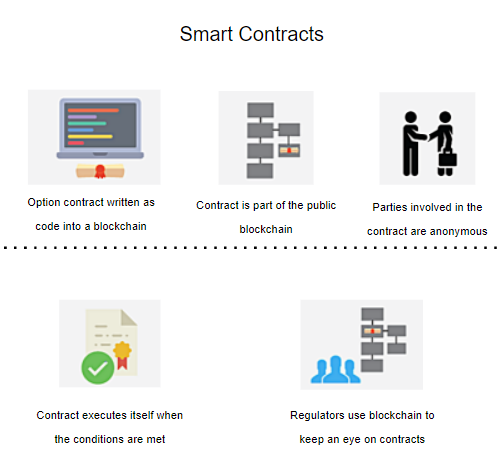
\includegraphics[width=0.6\textwidth, alt={Come funziona uno Smart Contract}]{immagini/smart-contract.png}
    \caption{Funzionamento di uno Smart Contract} \label{fig:smart-contract}
\end{figure}

Possiamo citare alcuni esempi di applicazione di smart contract:
\begin{itemize}
    \item \textit{smart legal contracts}, legalmente applicabili e richiedono alle parti di soddisfare i loro obblighi contrattuali.
    Per creare alcuni contratti legali intelligenti, le parti coinvolte lavorano sul codice del contratto intelligente - o lo fanno i loro sviluppatori di software - finché non si accordano sui termini e sulle condizioni dell'accordo;
    \item \textit{decentralized autonomous organizations (DAO)}, che sono organizzazioni che funzionano in modo decentralizzato e autonomo, senza un leader centrale e open-source, ma regolate da un contratto intelligente.
    All'interno delle blockchain vengono organizzate delle votazioni, che possono essere eseguite da tutti i partecipanti, che possono votare per o contro una proposta,
    oppure garantire il corretto scambio dei beni digitali all'interno della piattaforma, prevenendo possibili vulnerabilità;
    \item \textit{crowdfunding}, che è un metodo di finanziamento di progetti e aziende, in cui le persone possono contribuire con denaro o beni, in cambio di un premio o di un prodotto finale;
    \item \textit{logical applicative contracts}, che sono contratti che possono essere utilizzati per eseguire operazioni logiche, come la verifica di un dato e l'esecuzione di un'altra operazione,
    oppure gestire un sistema di pagamento o beni di scambio, garantendo la tracciabilità e la trasparenza di ogni bene alla consegna.
\end{itemize}

I contratti rimangono aggiornati grazie all'uso di \textit{oracoli}, sistemi che permettono di ottenere informazioni esterne alla blockchain, come il valore di un bene o il valore di un'azione,
attraverso l'uso di API o di altri sistemi di comunicazione. In questo modo, il contratto mantiene la sua funzionalità interagendo in maniera ibrida con il mondo esterno; questi vengono definiti come \textit{hybrid smart contracts}, 
combinando un'infrastruttura \textit{on-chain} con un'infrastruttura \textit{off-chain}.
Il loro utilizzo, per quanto utile, deve essere attentamente bilanciato, sia in termini di veridicità dei dati che di sicurezza, in quanto possono essere soggetti a compromissione o di scalabilità, per cui è necessario
un'attenta valutazione dei rischi.

\subsection{Scalabilità}\label{sec:tecnologie-blockchain-avanzate-scalabilita}
Le blockchain sono preziose per il fatto di essere un sistema deterministico e con un grado di affidabilità molto elevato, generalmente neutro e verificabile da parte dell'utente finale.
In questo contesto, è fondamentale parlare del cosiddetto \textit{blockchain trilemma}, che è un problema di scelta tra tre caratteristiche fondamentali di una blockchain: decentralizzazione, sicurezza e scalabilità.
Infatti, decentralizzare significa mantenere un vasto numero di nodi sulla rete, senza però alcun controllo da parte di un ente centrale, 
mantenendo allo stesso modo un alto numero di transazioni in modo scalabile e una robustezza ai possibili partecipanti della rete. \\

In questo senso, si cerca di trovare un compromesso tra le tre caratteristiche, che è possibile ottenere l'aggiunta di ridondanza dei dati anche al di fuori della blockchain principale,
cercando di bilanciare quanto possibile il consenso sui nodi distribuiti non intaccando il livello di libertà offerto ma anche aumentare il livello di dati trasmessi.
Per questo, il nucleo scalabilità permette di introdurre numerose soluzioni al fine di migliorare le prestazioni della blockchain, dividendo però la blockchain in vari strati, definiti come \textit{layer}.
\begin{itemize}
    \item{\textit{Layer 0}}, che è la blockchain principale, che contiene i dati e le transazioni;
    \item{\textit{Layer 1}}, che è il livello responsabile della sicurezza e della scalabilità, che contiene i nodi che eseguono le transazioni e che sono responsabili della validazione;
    \item{\textit{Layer 2}}, noto anche come livello di esecuzione, in cui si hanno i contratti intelligenti e le applicazioni che vengono eseguite sulla blockchain;
    \item{\textit{Layer 3}}, noto anche come livello applicativo, che contiene le applicazioni decentralizzate (dApps), eseguite sulle blockchain e che interagiscono con gli utenti.
\end{itemize}

Comunemente, le soluzioni di scalabilità cercano di intervenire in vari modi:
\begin{itemize}
    \item{\textit{Sharding}}, che è una tecnica di scalabilità che consente di dividere la blockchain in più parti, chiamate \textit{shards}, che possono essere gestite da nodi diversi e aumentando
    la dimensione dei singoli blocchi e la loro frequenza di creazione. Questa si effettua comunemente per il Layer 1.
    \item{\textit{Sidechains}}, che sono blockchain secondarie che vengono utilizzate per eseguire transazioni parallele, che vengono poi sincronizzate con la blockchain principale.
    In questo ambito, soluzioni comuni includono i \textit{canali di stato (state channels)}, che sono dei contratti intelligenti che permettono di eseguire transazioni tra due parti, senza che queste siano visibili sulla blockchain principale,
    e i \textit{canali di pagamento (payment channels)}, che migliorano la comunicazione bidirezionale delle transazioni eseguendole sulla blockchain secondaria e dandone traccia sulla principale.
\end{itemize}

\newpage

\section{Self-Sovereign Identity}\label{sec:self-sovereign-identity}

La \glsfirstoccur{\gls{ssig}} è un approccio all'identità digitale che dà agli individui 
il controllo sulle informazioni che usano per dimostrare chi sono a siti web, servizi e applicazioni in tutto il web. 
Senza l'SSI, gli individui con account (identità) persistenti su Internet devono affidarsi a una serie di fornitori terzi, come Facebook, Google e altri,
che hanno il controllo delle informazioni associate alla loro identità. \\

Esistono molti modi per implementare l'SSI utilizzando le chiavi crittografiche e ne analizzeremo due.
\begin{itemize}
    \item l'utilizzo di firme digitali, attraverso un processo di \textit{firma digitale}, che permette di firmare un documento con una chiave privata, e di verificare la firma con la chiave pubblica;
    \item \glsfirstoccur{\gls{didg}}, che è un identificatore univoco alfanumerico per un soggetto, che può essere utilizzato per identificare una persona, un'organizzazione, un dispositivo, un servizio, un documento, ecc.
\end{itemize}  

Le parti coinvolte in questo processo sono principalmente tre:
\begin{enumerate}
    \item {\textit{emittente}, detto anche \textit{holder}}, ossia l'entità che emette una credenziale, ad esempio un documento d'identità governativo;
    \item {\textit{titolare}, detto anche \textit{issuer}}, ossia il proprietario della credenziale, cioè l'entità su cui l'emittente genera la credenziale;
    \item {\textit{verificatore}, detto anche \textit{verifier}}, cioè l'entità che controlla la validità e l'autenticità della credenziale presentata dal titolare.
\end{enumerate}  

Il processo di riconoscimento è descritto dalla figura \ref{fig:ssi}.

\begin{figure}[h]
    \centering
    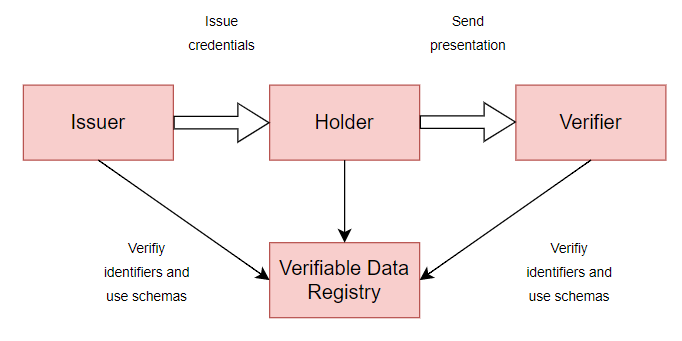
\includegraphics[width=0.6\textwidth, alt={Come funziona il riconoscimento nella SSI}]{immagini/ssi.png}
    \caption{Processo di riconoscimento di una credenziale SSI} \label{fig:ssi}.
\end{figure}

Lo scopo principale di questa tecnologia è consentire agli utenti un'esistenza indipendente da provider terzi, 
permettendo loro di controllare la propria identità in modo sicuro e accedendovi senza dover affidarsi a terzi. \\
Inoltre, i sistemi e gli algoritmi che la supportano devono essere trasparenti, mantenendo le informazioni in modo trasparente e permanente, rendendo però semplice 
la portabilità e l'interoperabilità di queste all'interno delle varie piattaforme. \\

La tecnologia blockchain, per mezzo della sua natura decentralizzata, permette di creare un sistema di identità digitale che soddisfi questi requisiti.
In particolare:
\begin{itemize}
    \item il titolare della credenziale possiede il suo DID firmato dalla propria coppia di chiavi che certifica la sua identità;
    \item l'emittente fornisce delle \glsfirstoccur{\gls{vcg}}, che certificano in modo digitale e crittograficamente protetto la validità del proprio ruolo;
    \item il verificatore controlla che, tramite ciascun blocco, sia stata rilasciata una VC valida e che il titolare sia il legittimo possessore di quella VC.
\end{itemize}  

L'obiettivo principale è quello di fornire un utilizzo delle tecnologie blockchain tali da permettere agli utenti 
di selezionare quali credenziali mostrare (\textit{selective disclosure o divulgazione selettiva}),
secondo opportuni standard definiti gradualmente dall'organizzazione internazionale \textit{W3C}, tra cui il citato VC.

\subsection{Tipi e applicazioni}\label{sec:self-sovereign-identity-tipi-applicazioni}

Il concetto di SSI è stato introdotto nel 2015 da Sovrin Foundation, che ha sviluppato il protocollo Sovrin,
organizzazione privata senza scopo di lucro che ha creato la prima rete di identità auto-sovrana, diventato poi standard W3C. 
Esso si basa sul protocollo è \textit{Hyperledger Indy}, che è un framework open source per la creazione di SSI basato su blockchain
che fornisce strumenti, librerie e componenti riutilizzabili per fornire identità digitali legate al mondo blockchain, 
come ad esempio la firma digitale e la crittografia. \\

Questo è il principale, ma possiamo definire un insieme di standard 
utilizzati al fine di garantire agli utenti di possedere e controllare in modo indipendente la propria identità digitale, gestendo come vengono
condivise le proprie informazioni. La particolarità di questi protocolli è di comunicare gli uni con gli altri attraverso messaggi crittografati:
\begin{itemize}
    \item \textit{DID (Decentralized Identifier)}, che consente di creare identificativi digitali decentralizzati come citato supportano
    e permettono di identificare i soggetti in modo resistente alla falsificazione, autenticando le informazioni in modo sicuro;
    \item \textit{VC (Verifiable Credentials)}, che consente di gestire attestazioni verificati, quindi insiemi di informazioni cfhe un individuo
    possiede o controlla, dimostrando che l'attestazione è stata rilasciata da un emittente autorizzato. Questo all'interno delle blockchain
    garantisce che ciascun nodo e parte in gioco sia chi dice di essere senza ledere la decentralizzazione alla base;
    \item \glsfirstoccur{\gls{zkpg}}, che consente di dimostrare la conoscenza di una proprietà di un dato, senza rivelare alcun dettaglio relativo.
    Questa tecnologia è considerata a sé stante un'innovazione tecnologica, che permette attraverso l'individuazione di parti precise,
    la certezza che solo chi conosce l'informazione può correttamente rispondere alle domande poste senza rivelare i propri dati.
\end{itemize}

Attualmente, la tecnologia SSI prevede una graduale implementazione in sistemi di autenticazione e
in generale di accesso ai servizi pubblici, permettendo all'utente un ulteriore controllo
sui dati trasmessi rivelandoli solo a parti autorizzate.
Questo risulta particolarmente utile nel settore sanitario, legislativo (garantendo certezza di identità e di voto) e finanziario,
permettendo di ridurre i costi di gestione e di mantenimento dei dati, oltre che di ridurre i tempi di accesso ai servizi.
Il principale organo promotore è la \textit{Decentralized Identity Foundation (DIF)}, che ha come obiettivo quello di creare
un ecosistema di identità digitali decentralizzate, promuovendo integrazioni, progetti e nuove idee in questo ambito. 

\section{Zero Knowledge Proof}\label{sec:zero-knowledge-proof}
Definita anche come prova a conoscenza zero, è una tecnologia che permette di dimostrare la conoscenza di una proprietà di un dato,
senza rivelare alcun dettaglio relativo.
Occorre definire le parti coinvolte:
\begin{itemize}
    \item \textit{Prover}, ossia l'entità che prova la conoscenza di alcune informazioni riservate. 
    L'informazione segreta è il `testimone' (\textit{witness}) della prova e la presunta conoscenza del testimone da parte del prover stabilisce un insieme di domande a cui può rispondere solo chi conosce l'informazione. 
    \item \textit{Verifier}, ossia l'entità che verifica la correttezza della prova. Lui si occupa di scegliere a caso la sfida (\textit{challenge}) e di verificare la risposta del prover.
    La risposta del prover permette al verificatore di controllare se il primo ha davvero accesso al testimone. La verifica segue visivamente dalla figura \ref{fig:zkp}. 
    Per assicurarsi che il prover non stia indovinando alla cieca e non ottenga le risposte corrette per caso, il verificatore sceglie altre domande da porre.
\end{itemize}

\begin{figure}[h] 
    \centering
    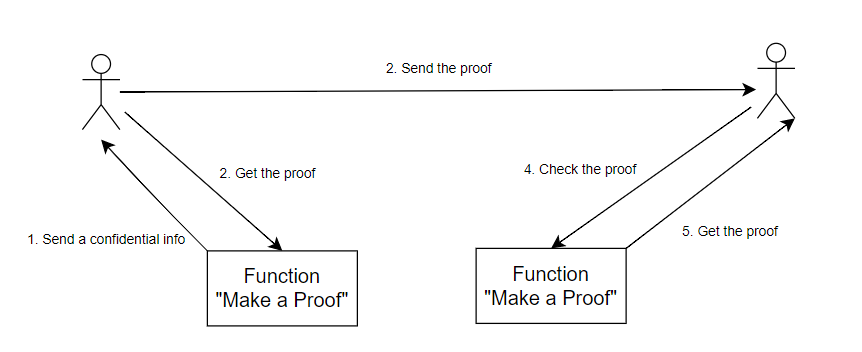
\includegraphics[width=0.6\textwidth, alt={Come funziona la verifica nella ZKP}]{immagini/zkp.png}
    \caption{Processo di verifica di una ZKP}\label{fig:zkp}
\end{figure}

A livello di transazioni, la ZKP è utilizzata per garantire la sicurezza con certezza che le transazioni siano valide (\textit{validity proofs}), tramite la presenza del testimone tipicamente basato su calcoli polinomiali o
prossimità ad un insieme di valori, come ad esempio la distanza di Hamming. Le transazioni possono essere invalidate in ogni momento tramite le \textit{fraud proofs}, che dimostrano che la transazione è stata effettuata in modo illegittimo.
Queste ultime confrontano i Merkle trees delle transazioni e verificano che l'hash corrisponda a quella originale. \\

Di fatto, ogni prova deve dimostrare di essere completa, pertanto è necessario che il verificatore sia in grado di verificare che la risposta del prover sia corretta,
dimostrando questa affermazione con solidità, in modo da non lasciare spazio a dubbi e a falsi positivi, senza trasmettere alcun dato (a conoscenza zero).
L'idea principale della ZKP è presupporre di non fidarsi di nessuno (\textit{zero trust}), al fine di garantire la sicurezza delle informazioni. 
In questo modo, ciascun utente viene monitorato a livello di privilegi, accessi e dati, senza che nessuno possa accedere senza dimostrare di averne il permesso. \\

\subsection{Tipi e applicazioni}\label{sec:zero-knowledge-proof-tipi-applicazioni}
Esistono diverse implementazioni di ZKP, ognuna delle quali presenta un proprio compromesso in termini di dimensione della prova, tempo del prover, tempo di verifica e altro ancora. 
I principali tipi sono: 
\begin{itemize}
    \item{\textit{zk-SNARK}}, acronimo di \textit{Zero Knowledge Succinct Non-interactive Argument of Knowledge}, prova di dimensioni ridotte e facile da verificare. Essa è stata sviluppata dalle piattaforme \textit{Zcash} e \textit{Ethereum} 
    utilizzando le curve ellittiche, che presuppongono che sia impossibile trovare il logaritmo discreto di un elemento casuale della curva ellittica a partire da un punto base pubblicamente noto. Il calcolo delle curve ellittiche è meno dispendioso dal punto di vista computazionale rispetto al calcolo delle funzioni di hashing.
    \item{\textit{zk-STARK}}, acronimo di \textit{Zero Knowledge Succinct Transparent Argument of Knowledge}, tipo di prova crittografica che richiede un'interazione minima o nulla tra il prover e il verificatore. I vantaggi principali delle STARK rispetto alle SNARK sono che hanno tempi di prover rapidi e sono più facili da scalare in quanto offrono una maggiore potenza di calcolo.
    Essa è stata sviluppata dalla piattaforma \textit{Horizen} utilizzando le \textit{curve ellittiche}, che presuppongono che sia impossibile trovare il logaritmo discreto di un elemento casuale della curva di Weierstrass a partire da un punto base pubblicamente noto. Il calcolo delle curve di Weierstrass è più dispendioso dal punto di vista computazionale rispetto al calcolo delle curve ellittiche.
\end{itemize}

All'interno delle blockchain, vengono utilizzati all'interno delle sidechain secondo il sistema delle \textit{zk-Rollup}, che permettono di eseguire transazioni su una blockchain laterale (sidechain) senza doverle scrivere su questa.
In altre parole, con uno zk-rollup, le transazioni vengono `confezionate' in un'unica transazione che viene elaborata sulla blockchain, riducendo il carico di lavoro richiesto alla rete. 
Inoltre, grazie all'utilizzo delle Zero Knowledge Proof, le transazioni vengono verificate in modo sicuro, senza rivelare alcuna informazione sulle transazioni stesse.

Principalmente, queste vengono utilizzate in sistemi di scalabilità layer-2, al fine di memorizzare solo il minimo numero previsto di transazioni (\textit{rollup}),
oppure memorizzando solamente un hash sulla catena per proteggere i dati del libro mastro (validium), oppure scegliere come salvarli per ogni transazine (\textit{volition}).
Alcuni casi d'uso possibili di applicazione di questa tecnologia possono essere:
\begin{itemize}
    \item{pagamenti anonimi}
    \item{protezione dell'identità}
    \item{autenticazione}
    \item{archiviazione di dati sensibili}
\end{itemize}

L'utilizzo combinato con la Self-Sovereign Identity è particolarmente interessante perché consente di garantire la privacy e la sicurezza delle informazioni personali degli utenti.
In particolare, è possibile garantire di conoscere le parti in gioco nella rete poiché verificate
in modo sicuro e privato tramite credenziali certificate, scegliendo anzi quali informazioni rivelare e senza
dover rivelare alcuno dei propri dati per dimostrare di possederli. 
    \chapter{Descrizione dello stage}\label{cap:descrizione-stage}

\intro{In questa sezione viene presentata un'analisi del percorso di stage, una descrizione dell'idea e delle tecnologie,
individuando possibili rischi e problematiche che potrebbero presentarsi durante lo svolgimento dello stesso.
Inoltre, viene fornita una panoramica degli obiettivi da raggiungere e della pianificazione delle ore di lavoro.}

\section{Introduzione al progetto e idea dello stage}\label{sec:introduzione-progetto}

Oggi più che mai è importante garantire la sicurezza dei propri dati e delle proprie informazioni, permettendo uno scambio sicuro
e protetto di dati sensibili tra due o più entità. Inoltre, è necessario garantire che le informazioni siano autentiche e non modificate,
per evitare che un utente malintenzionato possa alterare i dati e compromettere la sicurezza del sistema.
Sulla base di questa premessa, in accordo con l'azienda, si è deciso di sviluppare un progetto che permetta di esplorare 
le possibili applicazioni della tecnologia \glsfirstoccur{\gls{blockchaing}} all'interno di un contesto reale e possibilmente applicabile in ambito aziendale. \\

In particolare, la piattaforma oggetto dello sviluppo durante il tirocinio ha come obiettivo principale il controllo dell'accesso ai contenuti
riservati, nel contesto dei film vietati ai minori. Grazie all'utilizzo della tecnologia \glsfirstoccur{\gls{blockchaing}} e dello standard \glsfirstoccur{\gls{w3cg}} \glsfirstoccur{\gls{ssig}},
permettendo quindi di riconoscere i propri utenti evitando condivisione di informazioni, ma criptando i propri dati personali e verificando l'autenticità
dei dati trasmessi. Il progetto si pone quindi di risolvere il problema della condivisione di contenuti riservati, tramite l'utilizzo di tecnologie innovative
e la collaborazione con lo stagista Alessio De Biasi, utilizzando il codice di un progetto di un laureando magistrale presso Computer Science
dell'Università Ca' Foscari richiamato come libreria e di altri stagisti di laurea triennale con progetti similari basati sull'applicazione di tecnologie immutabili e decentralizzate. \\

Il suo utilizzo è molto simile ad altre piattaforme basate sulla condivisione e prenotazione di contenuti multimediali legati ai film:
l'utente si registra presso la piattaforma, fornendo i propri dati personali e la propria età. In questa fase, si ha il riconoscimento dell'utente
tramite l'utilizzo di un \glsfirstoccur{\gls{didg}} e la creazione di un \glsfirstoccur{\gls{vcg}} contenente i dati personali dell'utente, che verrà poi utilizzato per l'autenticazione
e la verifica dei dati. Una volta effettuata la registrazione, l'utente può accedere alla piattaforma e visualizzare i contenuti disponibili, permettendo l'accesso
anche a contenuti limitati qualora l'utente sia maggiorenne. Riconosciuta l'età dell'utente e verificata dalla piattaforma blockchain la sua autenticità,
l'utente può visualizzare il contenuto selezionato dimostrando tramite \glsfirstoccur{\gls{zkpg}} di essere maggiorenne, senza dover fornire ulteriori informazioni personali,
completando la prenotazione. \\

Nello specifico, il progetto è sviluppato da autodidatta, chiedendo consigli e supporto allo stagista De Biasi per confronti e chiarimenti sull'implementazione degli standard in oggetto
e per l'utilizzo del codice dello \textit{smart contract} da lui fornito, usato come libreria per l'implementazione della piattaforma in oggetto.
Inoltre, consigli e supporto sono stati forniti anche in modo reciproco con lo stagista Raffaele Bussolotto, studente presso Ingegneria Informatica di Padova,
con un percorso simile al mio a livello di argomenti, basato sempre sulle tecnologie in oggetto ma con diverso scopo. 
Il loro supporto è stato puramente di confronto, in quanto l'implementazione dei rispettivi progetti è stata fatta in modo indipendente e senza collaborazione diretta. \\
Sulla base di queste premesse nasce il progetto \textbf{VerifiedMovies}.

\section{Analisi preventiva dei rischi}\label{sec:analisi-rischi}

Durante la fase di analisi iniziale sono stati individuati alcuni possibili rischi 
a cui si potrà andare incontro. Si è quindi proceduto a elaborare delle possibili soluzioni per far fronte a tali rischi. \\

\begin{risk}{Inesperienza tecnologica e metodologica} 
    \newline
    \riskdescription{il progetto prevede l'utilizzo di tecnologie e metodologie di cui non si ha piena esperienza e conoscenza, 
    rendendo più difficoltosa la comprensione e l'applicazione delle stesse in fase di implementazione}
    \risksolution{ è stato previsto un periodo di formazione iniziale per studiare le tecnologie e le metodologie da utilizzare
    e l'aiuto/supporto del tutor aziendale e di altri stagisti nella risoluzione di problemi e nella discussione di possibili soluzioni}\label{risk:inesperienza-tecnologica} 
\end{risk}

\medskip

\begin{risk}{Difficoltà di integrazione con lo smart contract da usare come libreria}
    \newline
    \riskdescription{il sistema potrebbe incontrare difficoltà nell'integrazione con lo smart contract da richiamare per la gestione delle identità digitali,
    a causa di errori di programmazione o di problemi di comunicazione tra le parti coinvolte}
    \risksolution{è stato previsto un periodo di test e debug per verificare il corretto funzionamento del sistema e per risolvere eventuali problemi riscontrati,
    approfondendo il dialogo con il tutor aziendale e con lo stagista che ha sviluppato lo smart contract che dovrà essere richiamato in fase di implementazione}\label{risk:integrazione-smart-contract}
\end{risk}

\medskip

\begin{risk}{Ritardi nello sviluppo}
    \newline
    \riskdescription{potrebbero verificarsi ritardi nello sviluppo del sistema a causa di problemi tecnici o imprevisti, come la mancanza di risorse necessarie o la complessità del progetto,
    rimodulando adeguatamente attività e tempistiche}\label{risk:ritardi-sviluppo}
    \risksolution{è stato previsto un periodo di test e debug per verificare il corretto funzionamento del sistema e per risolvere eventuali problemi riscontrati,
    intensificando il dialogo interno con il proponente e gli stagisti per discutere di possibili soluzioni e rimodulando le attività e le tempistiche in base alle necessità}
\end{risk}

\medskip

\begin{risk}{Problemi di sicurezza}
    \newline
    \riskdescription{il sistema potrebbe riscontrare problemi di sicurezza e vulnerabilità a attacchi informatici o la mancanza di protezione dei dati sensibili}
    \risksolution{fin dall'inizio dell'attività di sviluppo, si cerca di garantire un'implementazione al passo con le \textit{best practices} previste dai linguaggi di programmazione utilizzate e lato web, 
    come l'utilizzo di librerie e framework aggiornati e sicuri, la validazione dei dati in input e la protezione da attacchi di tipo \textit{SQL injection} e \textit{XSS}. Inoltre, è possibile prevedere un'attività di testing approfondito,
    ad esempio utilizzando strumenti di analisi statica del codice e di penetration testing, per verificare la corretta implementazione delle misure di sicurezza e la presenza di eventuali vulnerabilità}\label{risk:problemi-sicurezza}
\end{risk}

\clearpage

\begin{risk}{Cambiamenti dei requisiti durante lo sviluppo}
    \newline
    \riskdescription{i requisiti del sistema potrebbero cambiare durante l'attività di implementazione, ad esempio a causa di una modifica delle esigenze del progetto o di un errore di analisi iniziale}
    \risksolution{è possibile prevedere un'attività di pianificazione flessibile, ad esempio utilizzando metodologie agili, come \glsfirstoccur{\gls{scrumg}}, che prevedono una pianificazione adattiva ai cambiamenti dei requisiti. 
    Inoltre, potrebbe essere utile prevedere una comunicazione costante con il tutor aziendale e gli altri stagisti in fase di validazione dei requisiti aggiornati, procedendo con lo sviluppo in modo coerente ed organizzato}\label{risk:cambiamenti-requisiti}
\end{risk}

\section{Obiettivi e requisiti}\label{sec:obiettivi-requisiti}

Il tirocinio prevede lo svolgimento dei seguenti obiettivi, riportando questa notazione, come dal documento \textit{Piano di Lavoro}:
\begin{itemize}
    \item O per i requisiti obbligatori, vincolanti in quanto obiettivo primario richiesto dal committente;
    \item D per i requisiti desiderabili, non vincolanti o strettamente necessari, ma dal riconoscibile valore aggiunto;
    \item F per i requisiti facoltativi, rappresentanti valore aggiunto non strettamente competitivo.
\end{itemize}
Le sigle precedentemente indicate saranno seguite da una coppia sequenziale di numeri, identificativo del requisito.

\begin{itemize}

    \item Obbligatori:
        \begin{itemize}
            \item \underline{\textit{O01}}: descrivere i concetti di base della \glsfirstoccur{\gls{blockchaing}}, tra cui la sua architettura, i nodi della rete, la crittografia e il consenso distribuito;
            \item \underline{\textit{O02}}: analizzare il concetto di \glsfirstoccur{\gls{smartcontractg}} e il linguaggio \glsfirstoccur{\gls{solidityg}}, con particolare attenzione alle vulnerabilità principali e alle tecniche per evitare errori di programmazione;
            \item \underline{\textit{O03}}: approfondire il funzionamento della firma asimmetrica delle transazioni su catena e la validazione dei blocchi, studiando le tipologie di consenso e le catene più conosciute;
            \item \underline{\textit{O04}}: studiare le tecniche di crittografia utilizzate per garantire la sicurezza e la \textit{privacy} delle informazioni personali nell'ambito della \glsfirstoccur{\gls{ssig}} e dei protocolli per la gestione delle identità digitali;
            \item \underline{\textit{O05}}: individuare casi d'uso reali per la \textit{Self Sovereign Identity}, analizzando i consorzi internazionali coinvolti in ambito di ricerca e i finanziamenti europei;
            \item \underline{\textit{O06}}: discutere le sfide e i problemi legati alla \textit{Self Sovereign Identity}, studiando un possibile scenario futuro di applicabilità e basato su \glsfirstoccur{\gls{zkpg}}.
        \end{itemize}

    \item Desiderabili:
        \begin{itemize}
            \item \underline{\textit{D01}}: implementare una \glsfirstoccur{\gls{dappg}} (o dApp) tramite le librerie \glsfirstoccur{\gls{ethersjsg}} oppure \glsfirstoccur{\gls{web3jsg}}, utilizzando uno smart contract di esempio;
            \item \underline{\textit{D02}}: realizzare una UI (interfaccia utente) per la dApp utilizzando \textit{HTML}, \textit{CSS} e \textit{JavaScript};
            \item \underline{\textit{D03}}: utilizzare la \textit{Self Sovereign Identity} e i protocolli studiati per implementare funzionalità di autenticazione utente nella dApp;
            \item \underline{\textit{D04}}: testare e debuggare l'applicazione implementata;
            \item \underline{\textit{D05}}: discutere problemi e sfide relativi all'implementazione di applicazioni decentralizzate su \textit{blockchain} \glsfirstoccur{\gls{ethereumg}}, con particolare attenzione alla scalabilità e alla sicurezza.
        \end{itemize}

    \item Facoltativi:
        \begin{itemize}
            \item \underline{\textit{F01}}: approfondire l'utilizzo di altri linguaggi di programmazione per gli \textit{smart contract}, come \textit{Vyper};
            \item \underline{\textit{F02}}: analizzare l'utilizzo di altre tecnologie \textit{blockchain}, come \textit{Polkadot} o \textit{Cardano}, per implementare la \textit{Self Sovereign Identity};
            \item \underline{\textit{F03}}: esplorare altre funzionalità delle librerie \textit{Ethers.js} e/o \textit{Web3.js}, come l'invio di transazioni;
            \item \underline{\textit{F04}}: investigare i limiti e le sfide legate all'utilizzo della tecnologia \textit{blockchain}.
        \end{itemize}
    
\end{itemize}
    \chapter{Analisi dei requisiti}
\label{cap:analisi-requisiti}

\intro{In questa sezione vengono analizzati i requisiti del progetto e ne viene data un'analisi ad alto livello, combinando una visione concettuale con una visione pratica ed implementativa. 
Vengono inoltre descritti i casi d'uso e i requisiti individuati, con l'obiettivo di fornire una visione generale del sistema e delle sue funzionalità, in modo semplice e comprensibile.}

\section{Descrizione ed analisi del sistema}
L'obiettivo del progetto è la creazione di una piattaforma per la visualizzazione di contenuti multimediali, in questo caso dei film,
tramite l'utilizzo degli standard \glsfirstoccur{\gls{w3cg}} \glsfirstoccur{\gls{didg}} e \glsfirstoccur{\gls{ssig}} per la verifica sicura dell'identità dell'utente e per la 
visualizzazione di tutti i contenuti della piattaforma, certificando in modo sicuro la propria identità senza diffondere dati personali tramite 
l'utilizzo di un \glsfirstoccur{\gls{zkpg}}.\\

Più precisamente, l'implementazione avviene usando lo \textit{smart contract} che implementa ad alto livello lo standard \glsfirstoccur{\gls{ssig}}, 
scritto nel linguaggio di programmazione \textit{Solidity} da parte dello studente magistrale Alessio De Biasi.
Questo contratto permette la gestione dell'identità digitale tramite la creazione di un documento di identità digitale, che contiene un identificatore univoco
chiamato \glsfirstoccur{\gls{didg}}, composto da una stringa alfanumerica che identifica l'utente, e un \textit{DID Document}, che contiene le informazioni dell'utente a lui associato.
Normalmente, la sua creazione avviene tramite un file \textit{json}, composto dallo standard di riferimento, l'identificativo ed un campo \textit{controller},
che ha la capacità di fare dei cambiamenti al documento stesso e certifica la firma digitale del documento, sulla base del metodo usato per la sua creazione.
Il formato del \textit{DID Document} è come il seguente (codice proveniente da \cite{site:didw3c}):

\begin{lstlisting}[language=json]
    {
      "@context": [
        "https://www.w3.org/ns/did/v1",
        "https://w3id.org/security/suites/ed25519-2020/v1"
      ]
      "id": "did:example:123456789abcdefghi",
      "authentication": [{    
        "id": "did:example:123456789abcdefghi#keys-1",
        "type": "Ed25519VerificationKey2020",
        "controller": "did:example:123456789abcdefghi",
        "publicKeyMultibase": "zH3C2AVvLMv6gmMNam3uVAjZpfkcJCwDwnZn6z3wXmqPV"
      }]
    }
\end{lstlisting}

\newpage

Nel codice che dovrà essere utilizzato come libreria,
ogni documento è caratterizzato da una \textit{capability delegation}, che permette di delegare l'accesso crittografico di un elemento ad un altro utente,
un servizio, specificando l'identificativo e l'indirizzo di un'entità autorizzata, un metodo di autenticazione, in cui viene stabilito
il modo in cui implementare il meccanismo di riconoscimento da parte dell'utente (dimostrando di fatto che sia chi dice di essere) e un 
genitore, composto da un identificativo ed una firma digitale.
L'idea del codice è di creare una cosiddetta `catena di fiducia', la cui idea è associare ad un utente un \glsfirstoccur{\gls{didg}} e dimostrare,
attraverso un meccanismo di autenticazione definito a priori nel documento tramite firme digitali, la risoluzione dei dati trasmessi, il riconoscimento univoco della sua identità
e l'accesso ad un determinato contenuto. Infatti, l'utente viene riconosciuto perché i suoi dati sono stati certificati da un ente 
con capacità di firma digitale che, a sua volta, si fida di altri enti anch'essi riconosciuti, fino ad arrivare ad un soggetto radice.
Se questa catena di fiducia viene risolta correttamente, l'utente viene riconosciuto univocamente e può accedere ai contenuti della piattaforma. \\

La struttura dati blockchain, attraverso l'utilizzo di un account associato ad un \glsfirstoccur{\gls{didg}}, permette di certificare l'identità dell'utente
tramite la firma digitale dei dati trasmessi con la propria coppia di chiavi pubblica/privata, certificando in modo immutabile la propria identità e
permette di realizzare un sistema di autenticazione sicuro e decentralizzato, che non richiede l'utilizzo di un ente terzo per la verifica delle informazioni. \\

L'utilizzo della piattaforma e delle sue parti prescinde dalla dimostrazione, attraverso una chiamata al contratto libreria fornito, della risoluzione attraverso firma digitale
del \glsfirstoccur{\gls{didg}} associato all'utente, che dimostra l'utilizzo di un account associato alla rete blockchain,
la sua identità. Se l'indirizzo che ha firmato digitalmente il documento è associato ad un profilo creatore di quel \glsfirstoccur{\gls{didg}} così firmato,
allora l'utente può accedere ai contenuti della piattaforma. L'implementazione di questo passaggio prevede che l'utente dimostri precisamente
la propria identità secondo un meccanismo \textit{challenge-response}: viene generato un numero casuale e viene chiesto all'utente di firmarlo digitalmente, in modo da dimostrare
che è in possesso della chiave privata associata all'indirizzo che ha firmato il documento. \\

Se il metodo di autenticazione conteneva la sua firma e come dato il numero casuale trasmesso, grazie alla generazione dell'identificatore
e la chiamata al contratto in grado di risalire precisamente all'account blockchain che l'ha emessa, si certifica l'utente in modo univoco.
Tale meccanismo viene implementato in fase di registrazione, in cui l'utente possiede un proprio \glsfirstoccur{\gls{didg}} e registra i propri dati anagrafici
e in fase di accesso, quando l'utente inserita esclusivamente come unico dato per effettuare il login il proprio identificatore, firmato digitalmente nella fase precedente e appartenente in modo univoco a lui. \\

In questa sezione, l'utente viene presentato ad un insieme di film e può scegliere di visualizzarne uno. Alla visualizzazione di un certo
contenuto oggetto a limiti di età, l'utente viene presentato ad una schermata di verifica, in cui deve dimostrare la sua età.
Questo passaggio avviene attraverso la creazione di una \glsfirstoccur{\gls{vpg}}, contenente molteplici \glsfirstoccur{\gls{vcg}}, 
con una associata all'utente (definito \textit{holder} delle credenziali) e le altre associate agli enti verificatori (definiti \textit{issuer}, che sono gli enti che hanno rilasciato le credenziali). \\

Normalmente, una \textit{Verifiable Presentation} è infatti composta da:
\begin{itemize}
    \item un insieme di metadati, che descrivono la presentazione;
    \item un insieme di \textit{Verifiable Credentials}, che sono le credenziali associate alla presentazione;
    \item un insieme di \textit{proof}, che sono le prove di autenticità delle credenziali.
\end{itemize}

Invece, una \textit{Verifiable Credential} è composta da:
\begin{itemize}
    \item un contesto di riferimento, che è un \textit{URI} che definisce il contesto di riferimento delle credenziali;
    \item un identificativo, che specifica il sito di riferimento;
    \item un tipo, che specifica se la credenziale è appropriata per la presentazione;
    \item un soggetto, che è l'identificativo dell'utente a cui sono associate le credenziali;
    \item un \textit{issuer}, che è l'identificativo dell'ente che ha rilasciato le credenziali;
    \item un \textit{issuanceDate}, che è la data di rilascio delle credenziali;
    \item una \textit{proof}, che è la prova di autenticità delle credenziali.
\end{itemize}

Il seguente è un esempio di una \textit{Verifiable Presentation} con al suo interno un insieme di \textit{Verifiable Credentials} (codice proveniente da \cite{site:vpw3c}):
\begin{lstlisting}[language=json]
    {
        "@context": [
          "https://www.w3.org/2018/credentials/v1",
          "https://www.w3.org/2018/credentials/examples/v1"
        ],
        "type": "VerifiablePresentation",
        "verifiableCredential": [
          {
            "@context": [
              "https://www.w3.org/2018/credentials/v1",
              "https://www.w3.org/2018/credentials/examples/v1"
            ],
            "type": ["VerifiableCredential", "UniversityDegreeCredential"],
            "credentialSchema": {
              "id": "did:example:cdf:35LB7w9ueWbagPL94T9bMLtyXDj9pX5o",
              "type": "did:example:schema:22KpkXgecryx9k7N6XN1QoN3gXwBkSU8SfyyYQG"
            },
            "issuer": "did:example:Wz4eUg7SetGfaUVCn8U9d62oDYrUJLuUtcy619",
            "credentialSubject": {
              "degreeType": "BachelorDegree",
              "degreeSchool": "College of Engineering"
            },
            "proof": {
              "type": "AnonCredDerivedCredentialv1",
              "primaryProof": "cg7wLNSi48K5qNyAVMwdYqVHSMv1Ur8i...Fg2ZvWF6zGvcSAsym2sgSk737",
              "nonRevocationProof": "mu6fg24MfJPU1HvSXsf3ybzKARib4WxG...RSce53M6UwQCxYshCuS3d2h"
            }
        }],
        "proof": {
          "type": "AnonCredPresentationProofv1",
          "proofValue": "DgYdYMUYHURJLD7xdnWRinqWCEY5u5fK...j915Lt3hMzLHoPiPQ9sSVfRrs1D"
        }
      }
\end{lstlisting}

Al suo interno, come si vede, sono presenti un insieme di credenziali, contenente un campo di dimostrazione di appartenenza ad uno schema comune,
a cui sarà associata la catena di fiducia, e degli insiemi di metodi di firma digitale, che dimostrano la validità delle credenziali presenti,
avendo ciascuna un insieme di \textit{issuer} riconosciuti. \\

Il meccanismo è in grado di integrarsi con \glsfirstoccur{\gls{zkpg}}, in cui la prova di appartenenza ad uno schema comune è dimostrata
senza rivelare informazioni sensibili di alcun tipo, combinando un insieme di \textit{Verifiable Credentials}, verificate tramite 
un insieme di \textit{issuer} riconosciuti dal sistema della catena di fiducia grazie all'uso della proprietà \textit{proof} descritta sopra
e la definizione di uno schema comune a cui fare riferimento, che certifica il riconoscimento in quanto firmato a catena da un insieme di \textit{issuer}
(secondo le specifiche dettagliate in \cite{site:zkpw3c}). \\
Questo permette all'utente di definire precisamente quali informazioni vuole rivelare e, attraverso l'utilizzo del contratto libreria, 
dimostrare la propria identità, verificato con questo meccanismo e accedendo al proprio contenuto di interesse. 

\section{Casi d'uso}

In questa sezione, saranno presenti un insieme di diagrammi dei casi d'uso, definiti secondo il linguaggio standard \glsfirstoccur{\gls{umlg}},
che descrivono le interazioni tra gli attori, definiti convenzionalmente come utenti del sistema e il sistema stesso. 
Seguirà una tabella di tracciamento dei requisiti, che mostrerà come i requisiti individuati nella sezione precedente siano soddisfatti
dai casi d'uso definiti in questa sezione, in base all'analisi prevista. \\

Di seguito, un diagramma complessivo (in figura \ref{fig:usecase-scenario-principale}) dei casi d'uso individuati, che verranno descritti nel dettaglio successivamente:

\begin{figure}[!h] 
    \centering 
    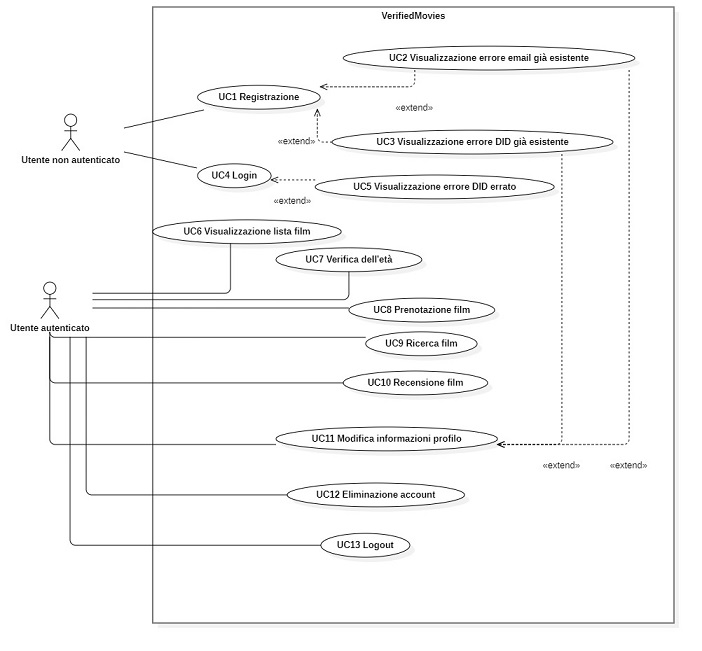
\includegraphics[width=0.9\columnwidth, alt={Scenario principale dei vari casi d'uso individuati}]{immagini/usecase/scenario-principale.jpg}
    \caption{Scenario principale}\label{fig:usecase-scenario-principale}
\end{figure}

\begin{usecase}{1}{Registrazione}\label{uc:registrazione}
\usecaseactors{Utente non autenticato}
\usecasepre{L'utente ha avviato l'applicazione web e ha aperto la pagina di registrazione}
\usecasedesc{L'utente vuole registrarsi presso l'applicazione web}
\usecasepost{L'utente ha completato la registrazione e può effettuare il login}
\usecasemain{L'utente: }

\begin{enumerate}
  \item inserisce il proprio username (UC1.1);
  \item inserisce la propria email (UC1.2);
  \item inserisce il proprio DID (UC1.3);
  \item inserisce la propria data di nascita (UC1.4).
\end{enumerate}

\usecaseext{}
\begin{enumerate}
  \item Visualizzazione errore email già esistente (UC2);
  \item Visualizzazione errore DID già esistente (UC3).
\end{enumerate}
\end{usecase}

\begin{figure}[!h] 
  \centering 
  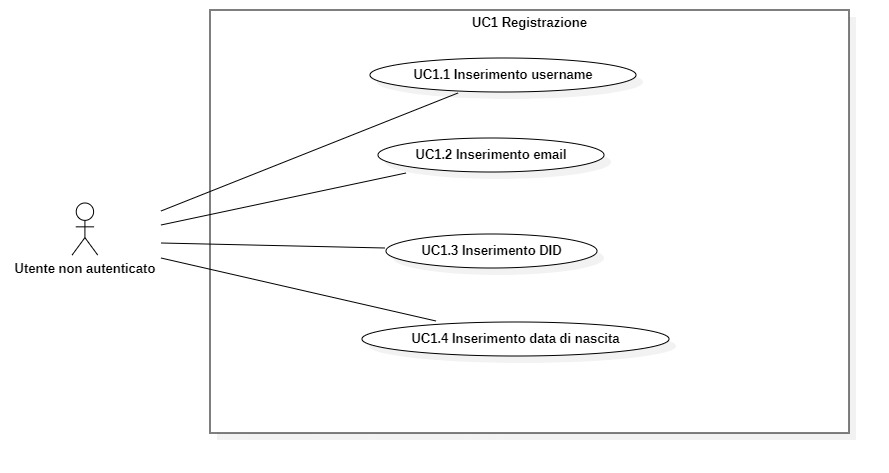
\includegraphics[width=0.9\columnwidth, alt={Caso d'uso relativo alla registrazione}]{immagini/usecase/UC1.jpg}
  \caption{UC1: Registrazione}\label{fig:uc:registrazione}
\end{figure}

\begin{usecase}{1.1}{Inserimento username}\label{uc:registrazione-username}
  \usecaseactors{Utente non autenticato}
  \usecasepre{L'utente ha avviato l'applicazione web e ha aperto la pagina di registrazione}
  \usecasedesc{L'utente deve inserire uno username per registrarsi presso l'applicazione web}
  \usecasepost{L'utente ha inserito lo username e può procedere con la registrazione}
  \usecasemain{}
  
  \begin{enumerate}
    \item L'utente inserisce il proprio username.
  \end{enumerate}
  
\end{usecase}

\begin{usecase}{1.2}{Inserimento email}\label{uc:registrazione-email}
  \usecaseactors{Utente non autenticato}
  \usecasepre{L'utente ha avviato l'applicazione web e ha aperto la pagina di registrazione}
  \usecasedesc{L'utente deve inserire una email per registrarsi presso l'applicazione web}
  \usecasepost{L'utente ha inserito la propria mail e può procedere con la registrazione}
  \usecasemain{}
  
  \begin{enumerate}
    \item L'utente inserisce la propria email.
  \end{enumerate}
  
\end{usecase}

\begin{usecase}{1.3}{Inserimento DID}\label{uc:registrazione-did}
  \usecaseactors{Utente non autenticato}
  \usecasepre{L'utente ha avviato l'applicazione web e ha aperto la pagina di registrazione}
  \usecasedesc{L'utente deve inserire il proprio DID per registrarsi presso l'applicazione web}
  \usecasepost{L'utente ha inserito il proprio DID e può procedere con la registrazione}
  \usecasemain{}
  
  \begin{enumerate}
    \item L'utente inserisce il proprio DID.
  \end{enumerate}
  
\end{usecase}

\begin{usecase}{1.4}{Inserimento data di nascita}\label{uc:registrazione-data}
  \usecaseactors{Utente non autenticato}
  \usecasepre{L'utente ha avviato l'applicazione web, non è autenticato e ha aperto la pagina di registrazione}
  \usecasedesc{L'utente deve inserire la propria data di nascita per registrarsi presso l'applicazione web}
  \usecasepost{L'utente ha inserito la propria data di nascita e può procedere con la registrazione}
  \usecasemain{}
  
  \begin{enumerate}
    \item L'utente inserisce la propria data di nascita.
  \end{enumerate}
  
\end{usecase}

\begin{usecase}{2}{Visualizzazione errore email già esistente}\label{uc:registrazione-email-esistente}
  \usecaseactors{Utente non autenticato}
  \usecasepre{L'utente ha inserito una email già esistente}
  \usecasedesc{L'utente deve inserire una email diversa per registrarsi presso l'applicazione web}
  \usecasepost{L'utente ha inserito una email diversa e può procedere con la registrazione}
  \usecasemain{}
  
  \begin{enumerate}
    \item L'utente visualizza un messaggio di errore che lo informa che la email inserita è già presente nel sistema.
  \end{enumerate}
\end{usecase}

\begin{usecase}{3}{Visualizzazione errore DID già esistente}\label{uc:registrazione-did-esistente}
  \usecaseactors{Utente non autenticato}
  \usecasepre{L'utente ha inserito un DID già esistente}
  \usecasedesc{L'utente deve inserire un DID diverso per registrarsi presso l'applicazione web}
  \usecasepost{L'utente ha inserito un DID diverso e può procedere con la registrazione}
  \usecasemain{}
  
  \begin{enumerate}
    \item L'utente visualizza un messaggio di errore che lo informa che il DID inserito è già presente nel sistema.
  \end{enumerate}
\end{usecase}

\begin{usecase}{4}{Login}\label{uc:autenticazione}
  \usecaseactors{Utente non autenticato}
  \usecasepre{L'utente ha avviato l'applicazione web, non è già autenticato e ha aperto la pagina di autenticazione}
  \usecasedesc{L'utente vuole entrare presso il sito e deve inserire le proprie credenziali per autenticarsi}
  \usecasepost{L'utente è autenticato correttamente e può procedere con l'utilizzo dell'applicazione}
  \usecasemain{}
  
  \begin{enumerate}
    \item L'utente inserisce il proprio DID.
  \end{enumerate}

  \usecaseext{}
  \begin{enumerate}
    \item Visualizzazione errore DID errato (UC5).
  \end{enumerate}
\end{usecase}

\begin{figure}[!h] 
  \centering 
  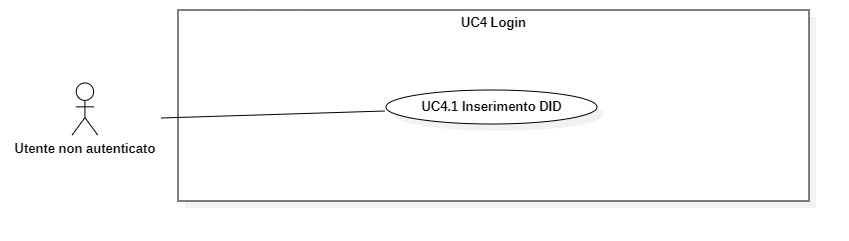
\includegraphics[width=0.9\columnwidth, alt={Caso d'uso relativo all'autenticazione dell'utente}]{immagini/usecase/UC4.jpg}
  \caption{UC4: Login}\label{fig:uc:autenticazione}
\end{figure}

\begin{usecase}{4.1}{Inserimento DID}\label{uc:autenticazione-did}
  \usecaseactors{Utente non autenticato}
  \usecasepre{L'utente ha avviato l'applicazione web, non è già autenticato e ha aperto la pagina di autenticazione}
  \usecasedesc{L'utente deve inserire il proprio DID associato alle proprie credenziali per autenticarsi presso l'applicazione web}
  \usecasepost{L'utente ha inserito il proprio DID e può procedere con l'autenticazione}
  \usecasemain{}
  
  \begin{enumerate}
    \item L'utente inserisce il proprio DID.
  \end{enumerate}

\end{usecase}

\begin{usecase}{5}{Visualizzazione lista film}\label{uc:visualizzazione-lista-film}
  \usecaseactors{Utente autenticato}
  \usecasepre{L'utente è autenticato e ha aperto la pagina principale dell'applicazione web}
  \usecasedesc{L'utente vuole visualizzare la lista dei film presenti nel sistema}
  \usecasepost{L'utente ha visualizzato la lista dei film presenti nel sistema}
  \usecasemain{}
  
  \begin{enumerate}
    \item L'utente visualizza la lista dei film presenti nel sistema.
  \end{enumerate}
\end{usecase}

\begin{figure}[!h] 
  \centering 
  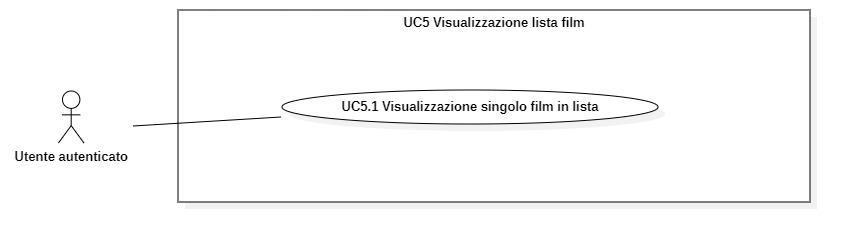
\includegraphics[width=0.9\columnwidth, alt={Caso d'uso relativo alla visualizzazione della lista dei film dell'utente}]{immagini/usecase/UC5.jpg}
  \caption{UC5: Visualizzazione lista film}\label{fig:uc:visualizzazione-lista-film}
\end{figure}

\begin{usecase}{5.1}{Visualizzazione singolo film in lista}\label{uc:visualizzazione-singolo-lista-film}
  \usecaseactors{Utente autenticato}
  \usecasepre{L'utente è autenticato e ha aperto la pagina principale dell'applicazione web}
  \usecasedesc{L'utente vuole visualizzare un singolo film dalla lista dei film presenti nel sistema}
  \usecasepost{L'utente ha visualizzato un film tra la lista di quelli presenti nel sistema}
  \usecasemain{}
  
  \begin{enumerate}
    \item L'utente visualizza un film tra quelli presenti nella lista del sistema.
  \end{enumerate}
\end{usecase}

\begin{usecase}{6}{Verifica dell'età}\label{uc:verifica-eta}
  \usecaseactors{Utente autenticato}
  \usecasepre{L'utente è autenticato, possiede una Verifiable Credential che attesta la sua età e intende visualizzare un film per prenotarlo} 
  \usecasedesc{L'utente vuole visualizzare un singolo film dalla lista dei film presenti nel sistema}
  \usecasepost{L'utente ha verificato la propria età in modo sicuro e può procedere con la prenotazione del film in oggetto}
  \usecasemain{}
  
  \begin{enumerate}
    \item L'utente seleziona un film dalla lista dei film presenti nel sistema;
    \item Il sistema prende la categoria di età del film selezionato e la confronta con l'età dell'utente.
    \item L'utente presenta la propria Verifiable Credential che attesta la sua età.
    \item Il sistema verifica la correttezza della Verifiable Credential utilizzando il DID del soggetto che l'ha rilasciata e genera una Verifiable Presentation contenente una Zero Knowledge Proof.
    \item Il sistema verifica la validità della Zero Knowledge Proof e verifica che l'età dell'utente sia maggiore o uguale a quella del film.
    \item Se la verifica ha successo, l'utente può procedere con la prenotazione del film.
  \end{enumerate}
\end{usecase}

\begin{usecase}{7}{Prenotazione film}\label{uc:prenotazione-film}
  \usecaseactors{Utente autenticato}
  \usecasepre{L'utente è autenticato, ha verificato la propria età e ha selezionato un film dalla lista dei film presenti nel sistema}
  \usecasedesc{L'utente vuole prenotare il film che ha selezionato dalla lista dei film presenti nel sistema}
  \usecasepost{L'utente ha verificato la propria età in modo sicuro e il film che ha selezionato è stato prenotato}
  \usecasemain{}
  
  \begin{enumerate}
    \item L'utente seleziona un film dalla lista dei film presenti nel sistema;
    \item Il sistema richiede all'utente di fornire i dettagli della prenotazione; 
    \item L'utente inserisce la data di prenotazione (UC7.1), l'orario di prenotazione (UC7.2) e il numero di posti da prenotare (UC7.3);
    \item Il sistema verifica la disponibilità del film per la data e l'orario selezionati e registra l'avvenuta prenotazione, fornendo un riepilogo all'utente.
  \end{enumerate}
\end{usecase}

\begin{figure}[!h] 
  \centering 
  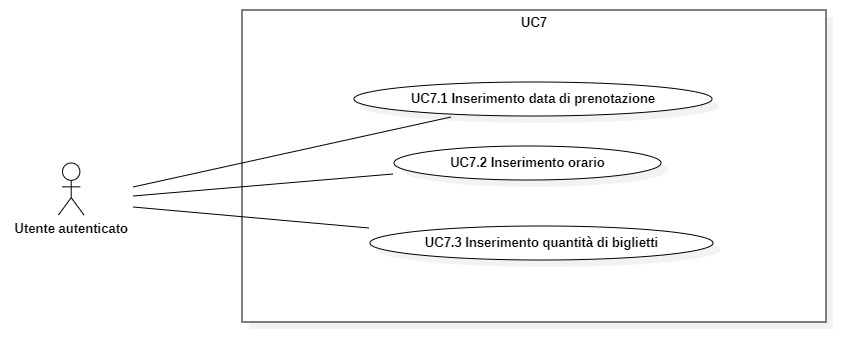
\includegraphics[width=0.9\columnwidth, alt={Caso d'uso relativo alla prenotazione di un film dell'utente}]{immagini/usecase/UC7.jpg}
  \caption{UC7: Prenotazione film}\label{fig:uc:prenotazione-film}
\end{figure}

\begin{usecase}{7.1}{Inserimento data prenotazione}\label{uc:inserimento-data-prenotazione}
  \usecaseactors{Utente autenticato}
  \usecasepre{L'utente è autenticato, ha verificato la propria età e ha selezionato un film dalla lista dei film presenti nel sistema}
  \usecasedesc{L'utente vuole inserire la data di prenotazione del film che ha selezionato dalla lista dei film presenti nel sistema}
  \usecasepost{L'utente ha inserito la data di prenotazione}
  \usecasemain{}
  
  \begin{enumerate}
    \item L'utente inserisce la data di prenotazione per il film che intende prenotare.
  \end{enumerate}
\end{usecase}

\begin{usecase}{7.2}{Inserimento orario prenotazione}\label{uc:inserimento-orario-prenotazione}
  \usecaseactors{Utente autenticato}
  \usecasepre{L'utente è autenticato, ha verificato la propria età e ha selezionato un film dalla lista dei film presenti nel sistema}
  \usecasedesc{L'utente vuole inserire l'orario di prenotazione del film che ha selezionato dalla lista dei film presenti nel sistema}
  \usecasepost{L'utente ha inserito l'orario di prenotazione}
  \usecasemain{}
  
  \begin{enumerate}
    \item L'utente inserisce l'orario di prenotazione per il film che intende prenotare.
  \end{enumerate}
\end{usecase}

\begin{usecase}{7.3}{Inserimento numero posti}\label{uc:inserimento-numero-posti}
  \usecaseactors{Utente autenticato}
  \usecasepre{L'utente è autenticato, ha verificato la propria età e ha selezionato un film dalla lista dei film presenti nel sistema}
  \usecasedesc{L'utente vuole inserire il numero di posti da prenotare per il film che ha selezionato dalla lista dei film presenti nel sistema}
  \usecasepost{L'utente ha inserito il numero di posti da prenotare}
  \usecasemain{}
  
  \begin{enumerate}
    \item L'utente inserisce il numero di posti da prenotare per il film che intende prenotare.
\end{enumerate}
\end{usecase}

\begin{usecase}{8}{Ricerca film}\label{uc:ricerca-film}
  \usecaseactors{Utente autenticato}
  \usecasepre{L'utente è autenticato}
  \usecasedesc{L'utente vuole cercare un film presente nel sistema e nel sistema sono presenti dei film}
  \usecasepost{L'utente ha cercato un film presente nel sistema e il sistema ha restituito i risultati della ricerca, permettendo all'utente di interagire con essi}
  \usecasemain{}
  
  \begin{enumerate}
    \item L'utente accede alla pagina principale contenente la lista dei film presenti nel sistema;
    \item L'utente inserisce il titolo del film che vuole cercare;
    \item Il sistema ricerca il film all'interno del sistema e restituisce i risultati della ricerca all'utente.
  \end{enumerate}
\end{usecase}

\begin{usecase}{9}{Recensione film}\label{uc:recensione-film}
  \usecaseactors{Utente autenticato}
  \usecasepre{L'utente è autenticato e visualizza la lista dei film prenotati}
  \usecasedesc{L'utente vuole recensire un film presente nel sistema}
  \usecasepost{L'utente ha recensito correttamente un film tra quelli presenti, anche senza prenotazione}
  \usecasemain{}
  
  \begin{enumerate}
    \item L'utente accede alla pagina principale contenente la lista dei film prenotati;
    \item L'utente seleziona il film che vuole recensire;
    \item L'utente inserisce la recensione del film;
    \item Il sistema registra la recensione del film e la associa all'utente che l'ha inserita.
  \end{enumerate}
\end{usecase}

\begin{usecase}{10}{Modifica informazioni profilo}\label{uc:modifica-informazioni-account}
  \usecaseactors{Utente autenticato}
  \usecasepre{L'utente è autenticato}
  \usecasedesc{L'utente vuole modificare le proprie informazioni personali}
  \usecasepost{L'utente ha modificato le proprie informazioni personali di proprio interesse}
  \usecasemain{}
  
  \begin{enumerate}
    \item L'utente accede alla pagina principale contenente le proprie informazioni personali;
    \item L'utente modifica il proprio username (UC10.1);
    \item L'utente modifica la propria email (UC10.2);
    \item L'utente modifica il proprio DID (UC10.3);
    \item L'utente modifica la propria data di nascita (UC10.4);
  \end{enumerate}

  \usecaseext{}
  \begin{enumerate}
    \item Visualizzazione errore email già esistente (UC2);
    \item Visualizzazione errore DID già esistente (UC3).
  \end{enumerate}
\end{usecase}

\begin{figure}[!h] 
  \centering 
  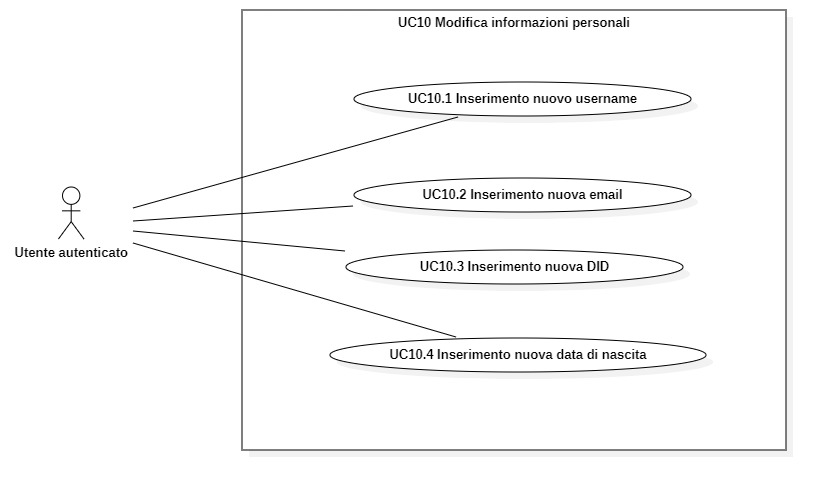
\includegraphics[width=0.9\columnwidth, alt={Caso d'uso relativo alla modifica delle informazioni del profilo}]{immagini/usecase/UC10.jpg}
  \caption{UC10: Modifica informazioni profilo}\label{fig:uc:prenotazione-film}
\end{figure}

\begin{usecase}{10.1}{Inserimento nuovo username}\label{uc:modifica-username}
  \usecaseactors{Utente autenticato}
  \usecasepre{L'utente è autenticato e intende modificare il proprio username}
  \usecasedesc{L'utente vuole modificare lo username associato al proprio account}
  \usecasepost{L'utente ha inserito il proprio username correttamente}
  \usecasemain{}
  
  \begin{enumerate}
    \item L'utente modifica il proprio username e conferma l'operazione.
  \end{enumerate}
  
\end{usecase}

\begin{usecase}{10.2}{Inserimento nuova email}\label{uc:modifica-email}
  \usecaseactors{Utente autenticato}
  \usecasepre{L'utente è autenticato e intende modificare la propria email}
  \usecasedesc{L'utente vuole modificare la mail associata al proprio account}
  \usecasepost{L'utente ha modificato la propria email correttamente}
  \usecasemain{}
  
  \begin{enumerate}
    \item L'utente modifica la propria email e conferma l'operazione.
  \end{enumerate}
  
\end{usecase}

\begin{usecase}{10.3}{Inserimento nuovo DID}\label{uc:modifica-did}
  \usecaseactors{Utente autenticato}
  \usecasepre{L'utente è autenticato e intende modificare il proprio DID}
  \usecasedesc{L'utente vuole modificare il DID associato al proprio account}
  \usecasepost{L'utente ha modificato il proprio DID correttamente}
  \usecasemain{}
  
  \begin{enumerate}
    \item L'utente modifica il proprio DID e conferma l'operazione.
  \end{enumerate}
  
\end{usecase}

\begin{usecase}{10.4}{Inserimento nuova data di nascita}\label{uc:modifica-data-nascita}
  \usecaseactors{Utente autenticato}
  \usecasepre{L'utente è autenticato e intende modificare la propria data di nascita}
  \usecasedesc{L'utente vuole modificare la data di nascita associata al proprio account}
  \usecasepost{L'utente ha modificato la data di nascita correttamente}
  \usecasemain{}
  
  \begin{enumerate}
    \item L'utente modifica la propria data di nascita e conferma l'operazione.
  \end{enumerate}
  
\end{usecase}

\begin{usecase}{11}{Eliminazione account}\label{uc:eliminazione-account}
  \usecaseactors{Utente autenticato}
  \usecasepre{L'utente è autenticato e intende eliminare il proprio account}
  \usecasedesc{L'utente vuole eliminare il proprio account dal sistema}
  \usecasepost{L'utente ha eliminato il proprio account e il sistema ha eliminato tutti i dati ad esso associati}
  \usecasemain{}
  
  \begin{enumerate}
    \item L'utente accede alla pagina principale contenente di modifica del profilo contenente le proprie informazioni personali;
    \item L'utente elimina il proprio account;
    \item Il sistema elimina l'account dell'utente, cancellando il DID e le informazioni ad esso associate.
  \end{enumerate}
\end{usecase}

\begin{usecase}{12}{Logout}\label{uc:logout}
  \usecaseactors{Utente autenticato}
  \usecasepre{L'utente è autenticato e intende uscire dalla propria sessione}
  \usecasedesc{L'utente vuole effettuare il logout dal sistema}
  \usecasepost{L'utente ha effettuato il logout e il sistema ha terminato la sessione dell'utente, non permettendo più l'accesso alle funzionalità riservate}
  \usecasemain{}
  
  \begin{enumerate}
    \item L'utente accede alla pagina principale contenente le proprie informazioni personali;
    \item L'utente effettua il logout;
    \item Il sistema effettua il logout dell'utente e l'utente è uscito dalla propria sessione.
  \end{enumerate}
\end{usecase}

\section{Tracciamento dei requisiti}

Da un'attenta analisi dei requisiti e degli use case effettuata sul progetto è stata stilata la tabella che traccia i requisiti in rapporto agli use case.\\
Sono stati individuati diversi tipi di requisiti e si è quindi fatto utilizzo di un codice identificativo per distinguerli.\\
Il codice dei requisiti è così strutturato R(F/Q/V)(N/D/O) dove:
\begin{enumerate}
	\item[R =] requisito
    \item[F =] funzionale
    \item[Q =] qualitativo
    \item[V =] di vincolo
    \item[N =] obbligatorio (necessario)
    \item[D =] desiderabile
    \item[Z =] opzionale
\end{enumerate}

Le fonti dei requisiti sono:
\begin{itemize}
  \item \textbf{UC} = use case
  \item \textbf{Interno} = requisito individuato dall'insieme di stagisti e tutor aziendali
\end{itemize}

Nelle tabelle \ref{tab:requisiti-funzionali}, \ref{tab:requisiti-qualitativi} e \ref{tab:requisiti-vincolo} sono riassunti i requisiti e il loro tracciamento con gli use case delineati in fase di analisi.

\newpage

\begin{table}%
\caption{Tabella del tracciamento dei requisiti funzionali}
\label{tab:requisiti-funzionali}
\begin{tabularx}{\textwidth}{lXl}
\hline\hline
\textbf{Requisito} & \textbf{Descrizione} & \textbf{Use Case}\\
\hline
RFN-1     & L'interfaccia permette di configurare il tipo di sonde del test & UC1 \\
\hline
\end{tabularx}
\end{table}%

\begin{table}%
\caption{Tabella del tracciamento dei requisiti qualitativi}
\label{tab:requisiti-qualitativi}
\begin{tabularx}{\textwidth}{lXl}
\hline\hline
\textbf{Requisito} & \textbf{Descrizione} & \textbf{Use Case}\\
\hline
RQD-1    & Le prestazioni del simulatore hardware deve garantire la giusta esecuzione dei test e non la generazione di falsi negativi & - \\
\hline
\end{tabularx}
\end{table}%

\begin{table}%
\caption{Tabella del tracciamento dei requisiti di vincolo}
\label{tab:requisiti-vincolo}
\begin{tabularx}{\textwidth}{lXl}
\hline\hline
\textbf{Requisito} & \textbf{Descrizione} & \textbf{Use Case}\\
\hline
RVO-1    & La libreria per l'esecuzione dei test automatici deve essere riutilizzabile & - \\
\hline
\end{tabularx}
\end{table}%

    \chapter{Progettazione e codifica}\label{cap:progettazione-codifica}

\intro{Breve introduzione al capitolo}

\section{Tecnologie utilizzate}\label{sec:tecnologie-strumenti}

In questa sezione, saranno elencate le tecnologie principali utilizzate durante lo sviluppo del sistema oggetto del tirocinio.

\subsection{Codifica}
\subsubsection{Solidity}

\subsubsection{ethers.js}

\subsubsection{web3.js}

\subsection{Versionamento}
\subsubsection{GitHub}

\section{Ciclo di vita del software}\label{sec:ciclo-vita-software}

\section{Progettazione}\label{sec:progettazione}

\subsubsection{Namespace 1} %**************************
Descrizione namespace 1.

\begin{namespacedesc}
    \classdesc{Classe 1}{Descrizione classe 1}
    \classdesc{Classe 2}{Descrizione classe 2}
\end{namespacedesc}


\section{Design Pattern Utilizzati}

\section{Codifica}

    \chapter{Verifica e validazione}\label{cap:verifica-validazione}
% chktex-file 1
% chktex-file 44

\intro{In questo capitolo verranno riportate le attività di verifica e validazione svolte durante lo sviluppo del progetto,
dettagliando i test svolti a tutti i livelli, dai test di unità fino alla fase di collaudo ed accettazione del prodotto}

\section{Accessibilità}\label{sec:verifica-validazione-accessibilita}

Al fine di rendere il sito più accessibile possibile, si è deciso di seguire le linee guida fornite da W3C, in particolare quelle riguardanti l'accessibilità dei contenuti web (WCAG) (\cite{site:wcag}), mantenendo il livello AA.\@
Questo ha comportato l'utilizzo di attributi \textit{alt} per le immagini di contenuto (lasciandolo vuoto per le immagini di presentazione) e l'utilizzo di attributi HTML semantici per la struttura del sito, come 
ad esempio \textit{<header>}, \textit{<main>}, \textit{<footer>} e \textit{<nav>} per gli elementi di navigazione, \textit{label} negli elementi dei form, \textit{<article>} per i contenuti principali della pagina.
Si riporta inoltre l'utilizzo degli attributi \textit{lang} per specificare la lingua del contenuto qualora fosse diversa dall'italiano. \\

Come descritto per la parte dei componenti, è stato creato un componente apposito per aiuto agli \textit{screen reader}, in grado di fornire un link per saltare la navigazione e accedere direttamente al contenuto principale della pagina
oppure l'opzione per tornare su in pagine grandi.
Il sito utilizza un layout a tre pannelli, cercando di rendere fluida l'esperienza di navigazione, evitando lo scorrimento laterale nelle condizioni di visualizzazione più comuni.
La struttura cerca di seguire un livello di intestazioni logiche, utilizzando \textit{<h1>} per il titolo principale della pagina, \textit{<h2>} per i titoli di sezione e \textit{<h3>} per i titoli di sottosezione,
tale da non saltare livelli di intestazione e consentire una navigazione più fluida nelle varie condizioni.
Il carattere utilizzato è \textit{Calibri}, un font \textit{sans-serif} che risulta essere mediamente ben leggibile, adottando convenzionalmente un'interlinea di 1.5 \textit{em} per migliorare la leggibilità del testo. \\

In merito ai contrasti utilizzati, le linee guida richiedono un rapporto di contrasto almeno pari a 4.5:1 per il testo normale e 3:1 per il testo grande, con alcune eccezioni per il testo in grassetto e per il testo non essenziale.
Con l'aiuto del sito \textit{WCAG Contrast Checker} (\cite{site:wcagcontrastchecker}) si è cercato di mantenere un livello di contrasto adeguato nelle varie situazioni, considerando lo sfondo, il testo e lo stato dei link di navigazione (visitato/non visitato) e dei bottoni (\textit{hover}/\textit{focus}).

In dettaglio, possiamo precisare:
\begin{itemize}
    \item per i contrasti nella pagina principale e per il testo nelle varie pagine, un colore con sfumatura \textit{\#ffffff80}, correttamente visibile rispetto all'immagine di sfondo;
    \item per i link di navigazione, un colore con sfumatura \textit{\#ffffff}, per lo stato di hover pari a \textit{\#ff8a8a}, lo stato di visitato con sfumatura \textit{\#ffec80}, tutti pienamente contrastanti con la barra di navigazione di colore \textit{\#141414}, usato qui e nel \textit{footer};
    \item per tutti i bottoni, il colore \textit{\#4c78a8}, per lo stato di hover il colore \textit{\#303f9f} e per lo stato di focus il colore \textit{\#3f51b580}, contrastanti con lo sfondo \textit{\#ffffff} delle finestre in cui sono usati.
\end{itemize}

Le convenzioni interne del sito, a livello grafico e di navigazione, sono state mantenute coerenti in tutte le pagine, cercando di rendere l'esperienza di navigazione più fluida possibile.
Ogni azione nel sito ha un apposito messaggio di \textit{feedforward} che indirizza l'utente sulle azioni che può compiere e sulle conseguenze che queste hanno, ricevendo un apposito \textit{feedback}.
Nella pagina con più contenuti è stata offerta un'opzione di ricerca per trovare più facilmente i contenuti desiderati, con un apposito messaggio di errore nel caso in cui non vengano trovati risultati.
A questo proposito, è stato utilizzato un componente apposito per la gestione degli errori, che permette di visualizzare un messaggio di errore e di tornare alla pagina precedente. \\

Le immagini utilizzate sono state ottimizzate in dimensione e peso, cercando di mantenere un livello di qualità adeguato, senza appesantire troppo il sito e il suo caricamento.
Le stesse ancore di navigazione hanno nomi esplicativi e sono state posizionate in modo da essere facilmente raggiungibili e cliccabili dall'apposita barra di navigazione.
Inoltre, si è deciso di evitare l'uso di tabelle, che possono risultare poco accessibili, e di utilizzare un layout a griglia per la disposizione dei contenuti grafici, offrendo come descritto in sezione~\ref{subsec:codifica-front-end} dei punti di rottura per ogni pagina per garantire la fruizione del sito anche su dispositivi mobili.
Un controllo generale di quanto descritto è stato effettuato con l'aiuto dell'estensione \textit{WAVE} (\cite{site:wave}), che ha permesso di individuare alcuni errori e avvisi, corretti e poi modificando di conseguenza,
portando il sito ad essere conforme alle linee guida definite. 

\section{Test di unità}\label{sec:verifica-validazione-test}

Qui vengono descritti i test di unità effettuati sul codice, utilizzando il framework \textit{Jest} (\cite{site:jest}), che permette di effettuare test di unità su codice \textit{JavaScript} e \textit{TypeScript}
e la libreria di test \textit{React Testing Library} (\cite{site:reacttestinglibrary}), che permette di effettuare test di unità su codice React.
Il codice identificativo dei test è strutturato da:
\begin{center}
    \textbf{TU[Numero]}
  \end{center}
\textbf{}
avendo come legenda:
\begin{itemize}
\item \textbf{TU}, cioè il test di unità, in grado di testare una singola unità di codice e di verificare che il suo comportamento sia corretto;
\item \textbf{Numero}, come numero identificativo univoco e progressivo del test in questione.
\end{itemize}

Ciascun test riporta le seguenti sigle:
\begin{itemize}
\item \textbf{I}: indica che il test è stato implementato e superato;
\item \textbf{NI}: indica che il test non è stato implementato.
\end{itemize}

Per una migliore comprensione del riferimento alle pagine e alle relativi componenti, con denominazione di riferimento in codifica, si rimanda 
alla sezione~\ref{subsec:codice-front-end}.

\renewcommand{\arraystretch}{1.1} % Adjust the spacing inside the cells

% Redefine column type to center the content
\newcolumntype{C}[1]{>{\centering\arraybackslash}p{#1}}

\begin{center}
\captionof{table}{Tabella di tracciamento dei test di unità}\label{tab:test-unita}
\begin{longtable}{|C{2.0cm}|C{3.0cm}|C{8.0cm}|C{2.0cm}|}
\hline
\textbf{ID} & \textbf{Elemento} & \textbf{Descrizione} & \textbf{Stato} \\
\hline
TU1 & AuthContext & Verificare se il componente AuthContext gestisce correttamente l'autenticazione, salvando lo stato dell'utente e fornendo la logica di autenticazione. & I \\
\hline
TU2 & Footer & Verificare se il componente Footer viene visualizzato e caricato correttamente in tutte le pagine dell'applicazione e se il link di ritorno funziona con screen reader. & I \\
\hline
\end{longtable}
\end{center}

\begin{center}
\begin{longtable}{|C{2.0cm}|C{3.0cm}|C{8.0cm}|C{2.0cm}|}
\hline
\multicolumn{4}{|c|}{\textbf{Continuazione della tabella~\ref{tab:test-unita}}} \\
\hline
\textbf{ID} & \textbf{Elemento} & \textbf{Descrizione} & \textbf{Stato} \\
\hline
\endhead
TU3 & NavBar & Verificare se il componente NavBar viene visualizzato e caricato correttamente in tutte le pagine dell'applicazione & I \\
\hline
TU4 & NavBar & Verificare se il componente NavBar permette la visualizzazione dei collegamenti corretti in base allo stato di autenticazione dell'utente & I \\
\hline
TU5 & PrivateRoute & Verificare se il componente PrivateRoute gestisce correttamente le rotte protette dell'applicazione, reindirizzando l'utente alla pagina di login se non è autenticato & I \\
\hline
TU6 & ScreenReaderHelp & Verificare se il componente ScreenReaderHelp è progettato correttamente per fornire supporto agli screen reader, rendendo il contenuto accessibile solo agli screen reader & I \\
\hline
TU7 & SearchBox & Verificare se il componente SearchBox gestisce correttamente la barra di ricerca dei film, effettuando la ricerca in base al titolo e aggiornando correttamente lo stato della ricerca & I \\
\hline
TU8 & Notification & Verificare se il componente Notification gestisce correttamente la visualizzazione degli errori e dei messaggi di notifica nelle diverse situazioni & I \\
\hline
% Aggiungi altre righe come necessario
\end{longtable}
\end{center}

\section{Test di integrazione}\label{sec:verifica-validazione-integrazione}

In questa sezione sono introdotti i test di integrazione, cioè la verifica del corretto funzionamento di più componenti del sistema, in grado di interagire tra loro.
Questo, in particolare, implica l'analisi del comportamento delle pagine e dei componenti grafici da cui sono composte.

Il codice identificativo dei test è strutturato da:
\begin{center}
    \textbf{TI[Numero]}
  \end{center}
\textbf{}
avendo come legenda:
\begin{itemize}
\item \textbf{TI}, cioè il singolo test di integrazione;
\item \textbf{Numero}, come numero identificativo univoco e progressivo del test in questione.
\end{itemize}

\begin{center}
\captionof{table}{Tabella del tracciamento dei test di integrazione}\label{tab:test-integrazione}
\begin{longtable}{|C{2.0cm}|C{3.0cm}|C{8.0cm}|C{2.0cm}|}
\hline
\textbf{ID} & \textbf{Elemento} & \textbf{Descrizione} & \textbf{Stato} \\
\hline
TI1 & HomePage & La pagina viene testata per verificarne il caricamento grafico e delle sue componenti & I \\
\hline
TI1 & HomePage & La pagina viene testata per verificare se le funzioni di creazione del DID e della catena degli issuer sono chiamate correttamente all'avvio dell'applicazione & I \\
\hline
\end{longtable}
\end{center}

\clearpage

\begin{center}
\begin{longtable}{|C{2.0cm}|C{3.0cm}|C{8.0cm}|C{2.0cm}|}
\hline
\multicolumn{4}{|c|}{\textbf{Continuazione della tabella~\ref{tab:test-integrazione}}} \\
\hline
\textbf{ID} & \textbf{Elemento} & \textbf{Descrizione} & \textbf{Stato} \\
\hline
\endhead
TI3 & RegisterView & La vista di registrazione viene testata per verificare che venga visualizzata correttamente & I \\
\hline
TI4 & RegisterView & La vista di registrazione viene testata per verificare che venga gestito correttamente il processo di registrazione tramite il meccanismo challenge-response & I \\
\hline
TI5 & RegisterView & La vista di registrazione viene testata per verificare che vengano gestiti correttamente i controlli di validazione dei campi e le notifiche di successo o di errore in caso di email o DID già registrati & I \\
\hline
TI6 & LoginView & La vista di login viene testata per verificare che venga visualizzata correttamente & I \\
\hline
TI7 & LoginView & La vista di login viene testata per verificare che venga gestito correttamente il processo di accesso tramite DID & I \\
\hline
TI8 & LoginView & La vista di login viene testata per verificare che vengano gestiti correttamente i controlli di validazione dei campi e le notifiche di errore in caso di DID non esistente & I \\
\hline
TI9 & LoginView & La vista di login viene testata per verificare che venga aperta correttamente la finestra modale di verifica dell'identità in caso di DID esistente & I \\
\hline
TI10 & LoginView & La vista di login viene testata per verificare che venga gestito correttamente il processo di verifica dell'identità & I \\
\hline
TI11 & MoviesView & La vista dei film viene testata per verificarne il caricamento grafico e delle sue componenti & I \\
\hline
TI12 & MoviesView & La vista dei film viene testata per verificare l'apertura di un film e la visualizzazione dei dettagli corretti & I \\
\hline
TI13 & MoviesView & La vista dei film viene testata per verificare l'apertura della finestra di verifica dell'età e il corretto funzionamento del processo di verifica & I \\
\hline
TI14 & MoviesView & La vista dei film viene testata per verificare la possibilità di condividere un film e l'apertura della finestra di condivisione & I \\
\hline
TI15 & MoviesView & La vista dei film viene testata per verificare la visualizzazione di un messaggio quando non ci sono film disponibili & I \\
\hline
\end{longtable}
\end{center}

\clearpage

\begin{center}
\begin{longtable}{|C{2.0cm}|C{3.0cm}|C{8.0cm}|C{2.0cm}|}
\hline
\multicolumn{4}{|c|}{\textbf{Continuazione della tabella~\ref{tab:test-integrazione}}} \\
\hline
\textbf{ID} & \textbf{Elemento} & \textbf{Descrizione} & \textbf{Stato} \\
\hline
\endhead
TI16 & MoviesView & La vista dei film viene testata per verificare la visualizzazione del profilo utente se autenticato & I \\
\hline
TI17 & MovieBookingView & La vista di prenotazione dei film viene testata per verificare che venga visualizzata correttamente & I \\
\hline
TI18 & MovieBookingView & La vista di prenotazione dei film viene testata per verificare che vengano inizializzati correttamente gli stati di prenotazione & I \\
\hline
TI19 & MovieBookingView & La vista di prenotazione dei film viene testata per verificare che venga gestito correttamente il processo di prenotazione & I \\
\hline
TI20 & MovieBookingView & La vista di prenotazione dei film viene testata per verificare che venga gestito il processo di visualizzazione del riepilogo della prenotazione in modo corretto & I \\
\hline
TI21 & MovieBookingView & La vista viene testata per verificare che venga gestito correttamente il processo di chiusura del modale di conferma prenotazione & I \\
\hline
TI22 & MovieBookingView & La vista viene testata per verificare che venga gestito correttamente il reindirizzamento alla pagina delle prenotazioni & I \\
\hline
TI23 & MovieBookingView & La vista viene testata per verificare che venga gestito il processo di validazione della prenotazione & I \\
\hline
TI24 & BookingListView & La vista di visualizzazione delle prenotazioni viene testata per verificare che venga renderizzata correttamente & I \\
\hline
TI25 & BookingListView & La vista di visualizzazione delle prenotazioni viene testata per verificare che venga mostrato il messaggio corretto quando non ci sono prenotazioni & I \\
\hline
TI26 & BookingListView & La vista di visualizzazione delle prenotazioni viene testata per verificare che vengano mostrate correttamente le prenotazioni presenti & I \\
\hline
TI27 & ErrorView & La vista di errore viene testata per verificare che venga renderizzata correttamente, riportando l'utente alla pagina principale & I \\
\hline
\end{longtable}
\end{center}

\clearpage

\section{Test di regressione}\label{sec:verifica-validazione-regressione}

Qui sono introdotti i test di regressione, cioè la verifica del corretto funzionamento del sistema dopo l'introduzione di modifiche, verificando di non aver 
introdotto errori in parti del sistema che precedentemente funzionavano correttamente.

Il codice identificativo dei test è strutturato da:
\begin{center}
    \textbf{TR[Numero]}
  \end{center}
\textbf{}
avendo come legenda:
\begin{itemize}
\item \textbf{TR}, cioè il singolo test di regressione;
\item \textbf{Numero}, come numero identificativo univoco e progressivo del test in questione.
\end{itemize}

\begin{center}
\captionof{table}{Tabella del tracciamento dei test di regressione}\label{tab:test-regressione}
\begin{longtable}{|C{2.0cm}|C{3.0cm}|C{8.0cm}|C{2.0cm}|}
\hline
\textbf{ID} & \textbf{Elemento} & \textbf{Descrizione} & \textbf{Stato} \\
\hline
TR1 & Applicazione & Si testa che l'applicazione venga correttamente caricata e visualizzata nelle sue funzionalità sul browser Google Chrome & I \\
\hline
TR2 & Applicazione & Si testa che l'applicazione venga correttamente caricata e visualizzata nelle sue funzionalità sul browser Microsoft Edge & I \\
\hline
TR3 & Applicazione & Si testa che l'applicazione venga correttamente caricata e visualizzata nelle sue funzionalità sul browser Safari & I \\
\hline
TR4 & Applicazione & Si testa che l'applicazione venga correttamente caricata e visualizzata nelle sue funzionalità sul browser Mozilla Firefox & I \\
\hline
TR5 & Applicazione & Si testa che l'applicazione venga correttamente caricata e visualizzata nelle sue funzionalità sul browser Opera & I \\
\hline
TR6 & MovieBookingView & Si verifica che le modifiche apportate alla vista di prenotazione non abbiano causato malfunzionamenti & I \\
\hline
TR7 & MoviesView & Si verifica che eventuali modifiche apportate al meccanismo di verifica della pagina non causino errori o malfunzionamenti compromettendo l'intera logica applicativa & I \\
\hline
TR8 & Applicazione & Si verifica che se vengono implementate modifiche al sistema di gestione di dati, l'applicazione sia comunque in grado di recuperarli correttamente & I \\
\hline
\end{longtable}
\end{center}

\clearpage

\section{Accettazione e collaudo}\label{sec:verifica-validazione-accettazione}

Settimanalmente, al fine di conoscere lo stato di avanzamento del prodotto, veniva organizzato un incontro interno con
il proponente e gli altri stagisti per discutere i progressi raggiunti e discutere eventuali dubbi o problemi riscontrati ad alto livello.
Ciò ha permesso di monitorare il lavoro e di conoscere lo stato dell'implementazione realizzata, garantendo così una maggiore
trasparenza e una migliore comunicazione tra le parti, permettendo di avere un feedback indicativo sulle attività da svolgere.
Alcuni chiarimenti si sono avuti con incontri autonomi con lo stagista magistrale Alessio De Biasi, di cui utilizzo il contratto come codice libreria 
per il funzionamento dell'applicazione. \\

Durante l'ultima settimana di stage, il proponente ha richiesto di effettuare un incontro per discutere del prodotto realizzato e per
mostrare l'applicazione completa e funzionante, dimostrando il raggiungimento degli obiettivi prefissati e delle funzionalità richieste, 
partendo dalle pagine ad alto livello e discutendo dei test e dei tipi di firma digitale e gli standard da me implementati. 
    \chapter{Conclusioni}\label{cap:conclusioni}

\intro{In questo capitolo verranno riportate le conclusioni del lavoro svolto, analizzando i risultati ottenuti e le conoscenze acquisite, 
analizzando i possibili sviluppi futuri degli amvbiti applicativi toccati dal progetto e dando una valutazione personale del lavoro svolto.}

\section{Obiettivi raggiunti e consuntivo finale}\label{sec:conclusioni-obiettivi-consuntivo}

In merito al raggiungimento degli obiettivi prefissati per il tirocinio (in sezione~\ref{sec:obiettivi-requisiti}),
si può confermare la soddisfazione di ciascuno. In particolare prima con lo studio e poi con la realizzazione dell'intero progetto,
i concetti di \glsfirstoccur{\gls{blockchaing}} e di \glsfirstoccur{\gls{smartcontractg}} sono stati acquisiti e compresi, dimostrando con la pratica la comprensione del
L'identità sovrana di \glsfirstoccur{\gls{ssig}} è stato applicato ed implementato in un contesto reale, con la possibilità di
interagire con un'applicazione web e con un'applicazione mobile, dimostrando la sua applicabilità in diversi ambiti.
Questo ha permesso, tramite lo studio e l'implementazione autonoma descritta di standard di identità e di firma digitale, di 
acquisire conoscenze e competenze in ambiti di sicurezza informatica e di crittografia, che sono stati approfonditi e studiati
in modo mirato nel progetto realizzato, garantendo la copertura dei requisiti obbligatori. \\

Più nello specifico, sono stati raggiunti correttamente i seguenti obiettivi obbligatori presenti da Piano di Lavoro di tirocinio:
\begin{itemize}
    \item \underline{\textit{O01}}: descrivere i concetti di base della \textit{blockchain} tra cui la sua architettura, i nodi della rete, la crittografia e il consenso distribuito;
    \item \underline{\textit{O02}}: analizzare il concetto di \textit{smart contract} e il linguaggio \glsfirstoccur{\gls{solidityg}}, con particolare attenzione alle vulnerabilità principali e alle tecniche per evitare errori di programmazione;
    \item \underline{\textit{O03}}: approfondire il funzionamento della firma asimmetrica delle transazioni su catena e la validazione dei blocchi, studiando le tipologie di consenso e le catene più conosciute;
    \item \underline{\textit{O04}}: studiare le tecniche di crittografia utilizzate per garantire la sicurezza e la \textit{privacy} delle informazioni personali nell'ambito della \textit{Self Sovereign Identity} e dei protocolli per la gestione delle identità digitali;
    \item \underline{\textit{O05}}: individuare casi d'uso reali per la \textit{Self Sovereign Identity}, analizzando i consorzi internazionali coinvolti in ambito di ricerca e i finanziamenti europei;
    \item \underline{\textit{O06}}: discutere le sfide e i problemi legati alla \textit{Self Sovereign Identity}, studiando un possibile scenario futuro di applicabilità e basato su \glsfirstoccur{\gls{zkpg}}.
\end{itemize}

Come richiesto dalla sezione degli obiettivi desiderabili presenti nella sezione citata, l'applicazione implementa la libreria 
\glsfirstoccur{\gls{web3jsg}} per l'interazione con la \textit{blockchain}, permettendo di interagire con lo \textit{smart contract} in modo corretto.
Inoltre, l'applicazione è stata completamente testata, come riportato dal capitolo~\ref{cap:verifica-validazione}. 
La stessa creazione dell'applicazione permette di esplorare uno scenario di applicazione dell'ambito della \textit{blockchain} e dell'identità connessa
senza trasmettere informazioni personali, risultando così in un'applicazione che rispetta la \textit{privacy} degli utenti.

\clearpage 

Più nello specifico, sono stati raggiunti i seguenti obiettivi desiderabili presenti nel Piano di Lavoro:
\begin{itemize}
    \item \underline{\textit{D01}}: implementare una \glsfirstoccur{\gls{dappg}} (o DApp) tramite le librerie \glsfirstoccur{\gls{ethersjsg}} oppure \glsfirstoccur{\gls{web3jsg}}, utilizzando uno \textit{smart contract} di esempio;
    \item \underline{\textit{D02}}: realizzare una UI (interfaccia utente) per la DApp utilizzando \textit{HTML}, \textit{CSS} e \textit{JavaScript};
    \item \underline{\textit{D03}}: utilizzare la \textit{Self Sovereign Identity} e i protocolli studiati per implementare funzionalità di autenticazione utente nella \textit{DApp};
    \item \underline{\textit{D04}}: testare l'applicazione implementata;
    \item \underline{\textit{D05}}: discutere problemi e sfide relativi all'implementazione di applicazioni decentralizzate su \textit{blockchain} \glsfirstoccur{\gls{ethereumg}}, con particolare attenzione alla scalabilità e alla sicurezza.
\end{itemize}

\section{Conoscenze acquisite e analisi del lavoro svolto}\label{sec:conclusioni-conoscenze-lavoro}

Il tirocinio svolto ha soddisfatto delle aspettative principalmente da un punto di vista conoscitivo, dato che ho capito le implicazioni del mondo \textit{blockchain} e come questo rappresenti,
se ben applicato, un passo importante da un punto di vista di sicurezza. 
Il punto più rilevante di questo tirocinio è stata certamente l'implementazione di questo progetto sfruttando un codice di un laureando magistrale, ampliando questa applicazione a degli standard \glsfirstoccur{\gls{w3cg}}
di non poca importanza, come \glsfirstoccur{\gls{didg}} e \glsfirstoccur{\gls{vcg}}, sviluppando una parte non completamente normata come \glsfirstoccur{\gls{zkpg}}. \\

L'attività è stata molto impegnativa e, nonostante il supporto di massima presente, la parte analitica e di effettivo sviluppo del progetto, specie della parte effettivamente più difficile come 
\textit{Zero Knowledge Proof} sono risultate estremamente teoriche e senza un vero supporto, se non da un punto di vista di puro ragionamento logico, da parte del laureando magistrale Alessio De Biasi, 
il progetto è risultato di difficile implementazione e comprensione autonoma, sia da un punto di vista di requisiti che di codifica vera e propria. Le scelte implementative e la loro realizzazione sono risultate attività pesanti e tediose, 
ma sono state comunque affrontate con successo e con determinazione, permettendomi di acquisire conoscenze e competenze in ambiti di sicurezza informatica e di crittografia decisamente importanti per un percorso di Laurea Triennale come il mio. \\

Di massima, è possibile descrivere le principali conoscenze maturate nell'ambito progettuale:
\begin{itemize}
    \item \textbf{comprensione dell'ambito \textit{blockchain} e sviluppo di \textit{smart contract}}: l'interazione di uno \textit{smart contract} e la sua interazione con un'applicazione web e mobile,
    permettono di comprendere come implementare una struttura dati pubblica ed immutabile, cambiando l'idea stessa di programmazione classica e facendo ben comprendere
    come ogni azione fatta in codice possa avere potenziali implicazioni di sicurezza. Ogni transazione è infatti pubblica e richiede una vera comprensione della struttura sottostante 
    e di come scrivere il codice in modo sicuro e corretto, per evitare perdite di dati o di denaro. In questo ambito, utile certamente l'apprendimento autonomo del linguaggio \textit{Solidity} e della libreria \textit{web3.js},
    che permettono di interagire con la \textit{blockchain} in modo semplice e adattando tale logica a quella di un'applicazione realmente utilizzabile;
    \item \textbf{analisi di standard di identità digitale e di protocolli di firma digitale}: l'implementazione di \textit{Decentralized Identifiers (DID)} e \textit{Verifiable Credentials (VC)} ha permesso di comprendere come sia possibile implementare un sistema di identità digitale
    partendo da implementazioni definite e preesistenti, tuttora sporadicamente applicate, ma con un ambito di applicazione molto ampio. Di fatto, in un mondo come quello odierno dove la \textit{privacy} rappresenta una giusta preoccupazione per gli utenti medi e per la stessa informatica,
    tale progetto dimostra come, in modo relativamente semplice, sia possibile certificare che l'utente sia chi dice di essere, senza trasmettere informazioni personali, ma solo una firma digitale, che può essere verificata da chiunque sul meccanismo di catena di fiducia
    creato e descritto. Il meccanismo di riconoscimento dell'autenticità delle informazioni trasmesse dall'utente ha richiesto una creazione personalizzata di quanto esistente in ambito sicurezza e \textit{blockchain}, creando un meccanismo conforme agli standard 
    e di facile utilizzo, data la complessità degli argomenti descritti e da me trattati, che richiedono una conoscenza approfondita di basi crittografiche, di sicurezza e di come implementare questi standard in modo corretto e concreto;
    \item \textbf{studio e analisi di \textit{Zero Knowledge Proof}}: la realizzazione e l'applicazione di \textit{Zero Knowledge Proof} è stata una delle parti più complesse da implementare, data la natura estremamente teorica della stessa e della 
    sua successiva applicazione, che richiede necessariamente, dati gli standard precedentemente descritti, la comprensione di standard di firma digitale spesso non accuratamente documentati e che richiedono di studiare a fondo gli standard di riferimento e una ricerca
    in gran parte teorica, ben maggiore di quella prevista da alcuni ambiti di studio, dato il tempo relativamente limitato di effettiva implementazione conforme agli standard.
    \item \textbf{nuove competenze di programmazione e progettuali}: l'analisi e la progettazione dei dettaglio di un'applicazione web e mobile, con l'implementazione di un \glsfirstoccur{\gls{backendg}} e di un \glsfirstoccur{\gls{frontendg}}hanno permesso di sviluppare ulteriormente le mie conoscenze apprese durante il corso di Ingegneria
    del Software, normando in modo più efficace le attività di codifica e di realizzazione della documentazione, risolvendo sul campo problemi progettuali ma anche concettuali presenti e sviluppando modifiche in modo agile, separando le responsabilità delle componenti e delle pagine, 
    migliorando così la manutenibilità e la comprensione del codice. 
    L'applicazione del linguaggio di programmazione \textit{TypeScript} unito alla comprensione di vulnerabilità legate al linguaggio \textit{Solidity} risulta utile nell'ulteriore comprensione e applicazione da un punto di vista di sviluppo di applicativi web e mobile, 
    analizzando in dettaglio le caratteristiche offerte da questi linguaggi e librerie e strutturando il codice attraverso \textit{design pattern} di riferimento e architetture utili da un punto di vista logico e di sviluppo attraverso la \textit{Continuous Integration} e la \textit{Continuous Delivery} (\cite{site:cicd}), così implementando modifiche in modo continuativo 
    e strutturato, a calendario e nel corso dell'intero progetto. 
\end{itemize}

\section{Scenari di applicabilità e sviluppi futuri}\label{sec:conclusioni-conoscenze-sviluppi}

L'applicazione sviluppata rappresenta un importante punto di partenza per lo sviluppo di un sistema di identità digitale decentralizzato, che può essere utilizzato in molti contesti reali, come ad esempio:
\begin{itemize}
    \item \textbf{pagamenti anonimi e sicuri}: l'implementazione di \textit{Zero Knowledge Proof} consente di rendere anonime le transazioni effettuate sulla \textit{blockchain}, permettendo di creare un sistema di pagamento decentralizzato, non divulgando informazioni personali ma anche 
    permettendo, data la sua natura pubblica ed immutabile, di riconoscere l'autenticità del pagamento effettuato, invalidando in ogni momento la possibilità di effettuare un doppio pagamento, che può essere verificato da chiunque sul meccanismo di catena di fiducia creato e descritto.
    In questo senso, molte banche cercano di interessarsi al mondo \textit{blockchain} per creare dei sistemi di pagamento \textit{KYC~- Know Your Customer}, che permette di sapere con certezza se l'utente è chi dice di essere, senza trasmettere informazioni personali, ma solo una firma digitale
    pubblicamente verificabile, prevenendo possibili problemi legati al riciclaggio di denaro in modo conforme agli standard;
    \item \textbf{protezione dell'identità ed autenticazione sicura}: il progetto realizzato permette all'utente di costruirsi un'identità digitale `sovrana', permettendo facilmente di compiere un autenticazione senza rivelare alcun dato personale, non dipendendo da piattaforme terze 
    e permettendo di autenticarsi in modo sicuro e conforme agli standard, verificato in modo dettagliato e privo di manipolazioni, partendo da un meccanismo di base come quello previsto;
    \item \textbf{protezione dei dati di archiviazione}: l'utilizzo di \textit{Zero Knowledge Proof} consente di rendere anonime le informazioni archiviate sulla \textit{blockchain}, permettendo di creare un sistema di archiviazione decentralizzato, proibendo a qualsiasi utente 
    non autorizzato di vedere i dati e potervi accedere, permettendo l'accesso alle informazioni solo chi è in grado di dimostrare la conoscenza dello `schema' di accesso comune tramite la presentazione di una credenziale sicura generata sul momento che attesta l'autenticità dell'utente
    e viene verificata secondo sistemi di firma digitale come quelli in oggetto. Nel caso in cui l'utente cerchi di manipolare questi dati, i meccanismi di firma digitale implementati sono in grado di riconoscere qualora 
    l'utente abbia tentato di modificare i dati, invalidando la firma e rendendo impossibile l'accesso ai dati.
\end{itemize}

In questo senso, esistono vari progetti europei che mirano a studiare e scoprire nuove tecnologie per la creazione di sistemi di identità digitale basati su \textit{blockchain}, partendo dal programma comune \textit{Horizon 2020} (\cite{site:horizon2020}),
che ha stanziato un \textit{budget} di 80 miliardi di euro per la ricerca e lo sviluppo delle tecnologie qui in oggetto nel periodo dal 2014 al 2020.
Possiamo citare ad esempio \textit{DECODE~- Decentralized Citizen Owned Data Ecosystem} (\cite{site:decode}), che mira a creare un'infrastruttura di dati decentralizzata e sicura per i cittadini europei
utilizzando tecnologie \textit{blockchain} e \textit{Self Sovereign Identity}, permettendo ad ogni utente di firmare digitalmente le informazioni di identità e condividerle solo con le parti autorizzate.
Un esempio ulteriore è \textit{IRMA~- I Reveal My Attributes} (\cite{site:irma}), sistema di identità digitale basato su \textit{blockchain} che utilizza una combinazione di tecnologie crittografiche mirate a garantire la sicurezza e la \textit{privacy} dei dati personali attraverso l'uso di un'applicazione mobile 
che funge da portafoglio digitale per l'identità dell'utente, generando una prova crittografica verificabile senza dover rivelare alcuna informazione personale. \\

In questo contesto, il meccanismo descritto si inserisce in modo naturale in progetti di questo tipo, inserendosi in parallelo e rappresentando su piccola scala un possibile punto di partenza per lo sviluppo di un sistema di identità digitale decentralizzato vero e proprio.
L'utilizzo parallelo di \textit{Zero Knowledge Proof} e \textit{Self Sovereign Identity} realizza un meccanismo di autenticazione e riconoscimento garantendo il completo controllo delle informazioni trasmesse e senza divulgare dati personali.
Data infatti una prova di autenticazione, l'utente prova la propria identità attraverso la presentazioni di credenziali pubbliche e firmate digitalmente; il meccanismo \textit{blockchain} consente di verificare la firma e quindi l'autenticità dell'utente
mentre i meccanismi di firma sottostanti permettono di riconoscere se l'utente è in grado di dimostrare la conoscenza di un segreto, senza rivelarlo, e quindi di accedere ai dati. \\

Lo scoglio più grande è dato dalla difficoltà di utilizzo di queste tecnologie, che richiedono un'infrastruttura di base che permetta di comprendere a fondo le implicazioni e i vantaggi che portano, ad oggi ancora largamente inesplorati e poco conosciuti, se non da un punto di vista teorico e di ricerca.
Le premesse sulla carta sono ottime: garantire agli utenti il livello di accesso minimo necessario, esponendo l'utente solo a ciò che è strettamente necessario, segmentando l'accesso e controllando l'autenticità delle sue operazioni.
In questo contesto, è fondamentale introdurre un sistema di crittografia sicuro, che garantisca l'implementazione di un sistema a conoscenza zero, in cui è possibile sapere con certezza che ci si può fidare di ciascun nodo presente sulla rete senza conoscere 
alcun dato dei singoli nodi, ma verificando tramite meccanismi riconosciuti e progressivamente standardizzati la loro identità. 
In un mondo in cui la protezione dei dati è diventata una preoccupazione rilevante anche per l'utente medio, occorre necessariamente cercare di stare al passo sfruttando dei meccanismi sicuri che non dipendono da terzi; la \textit{blockchain} riesce a garantire questo livello di sicurezza,
permettendo di creare un sistema di identità digitale decentralizzato e sicuro, in cui l'utente è l'unico detentore delle proprie informazioni e può decidere in autonomia a chi e quando concedere l'accesso. \\

A livello infrastrutturale, è necessario creare dei sistemi che siano in grado di sostenere un sistema di questo tipo, che richiede un'infrastruttura di base basata su \textit{blockchain}, di per sé dispendiosa da un punto di vista energetico e computazionale in modo consistente rispetto a sistemi più tradizionali.
Inoltre, andrebbe certamente standardizzata in maniera rilevante: ad oggi esistono alcune norme ISO che descrivono i termini e le definizioni di base, ma non esistono ancora standard che definiscano in modo chiaro e preciso i meccanismi di autenticazione e di firma digitale,
in larga parte molto teorici in ambito crittografico e non ancora applicati in modo pratico. Legalmente infatti si sta cercando di equiparare questi sistemi a quelli tradizionali, ma data la stessa natura decentralizzata di questo mondo, è difficile trovare un punto di riferimento
univoco ed eticamente accettabile per tutti, come per il mondo dell'intelligenza artificiale. Come per quest'ultimo, rimane principalmente uno strumento in grado potenzialmente di garantire una sicurezza ben maggiore di quella di altri sistemi esistenti ed in grado 
di garantire il vero anonimato nel mondo della rete e di venire incontro egualmente agli utenti finali e alle aziende. 

\section{Valutazione personale}\label{sec:conclusioni-valutazione}

L'attività di stage si è rivelata molto utile per la crescita personale e professionale, permettendo di acquisire nuove conoscenze
e competenze in ambiti di sicurezza informatica e di crittografia, che sono stati approfonditi e studiati in modo mirato nel progetto realizzato.
Inoltre, l'ambito \textit{blockchain} è stato studiato in modo approfondito, permettendo di esplorare in autonomia un campo con ripercussioni
decisamente interessanti nel mondo dell'informatica, decisamente non visti né praticati in corsi universitari ed è stata un'esperienza assolutamente rilevante. 
Ho potuto in questo ambito confrontarmi su aspetti interessanti che offrono nuove prospettive in ambito di sicurezza e che danno una visione delle tecnologie informatiche più consapevole. \\

Spesso ambiti sconosciuti possono essere rilevanti da un punto di vista professionale, e questo è stato un esempio di come
andare oltre i preconcetti dati da un ambito ampiamente teorico e non ormato, si riveli in realtà un'occasione di crescita
e di apprendimento, richiedendo necessariamente di praticare a fondo uno studio mirato delle attività svolte. 
In questi casi, la passione per il conoscere guida e anticipa la necessità di apprendere, dando un'importante possibilità di conoscere e maturare,
altrimenti non offerta in modo così vicino alle realtà aziendali e future rimanendo in ambito puramente accademico.
L'attività di supporto è comunque stata presente di massima, dando ampia possibilità di sviluppo e organizzazione in modo autonomo, 
rimanendo vicino a me come studente e alle mie necessità. \\

Il progetto per me rappresenta una crescita che matura quanto compreso e visto in questi ultimi anni, permettendo di applicare in modo nuovo 
concetti per la maggior parte sconosciuti e con tecnologie nuove, calandomi in un contesto attuale e futuro, usando delle librerie specifiche e sviluppando un
pensiero critico nell'analisi, affinando ulteriormente una visione d'insieme dei corsi fin qui frequentati nel mio percorso di Laurea Triennale, perfezionando il mio metodo di studio 
ed il mio modo di affrontare un progetto di codifica con ripercussioni attuali e future in modo così intenso, completando quanto realizzato nel corso di Ingegneria del Software
e usando tali metodologie per affrontare e suddividere il lavoro in modo autonomo, partendo da quanto appreso in questi mesi.
Quanto studiato rappresenta un importante partenza per il mio futuro percorso di Laurea Magistrale, adattando già ora un codice oggetto di tesi da parte di un laureando magistrale,
ampliando delle competenze trasversali certamente utili per il mio futuro, accademico e non, ed aggiornandomi su un ambito decisamente attuale e di sicuro interesse per possibili sviluppi futuri.

    \appendix
    \chapter{Appendice A}

\epigraph{Citazione}{Autore della citazione}


    \backmatter
    \printglossary[type=\acronymtype, title=Acronimi e abbreviazioni, toctitle=Acronimi e abbreviazioni]
    \printglossary[type=main, title=Glossario, toctitle=Glossario]

    \cleardoublepage
\chapter{Bibliografia}

\nocite{*}

% Print book bibliography
\printbibliography[heading=subbibliography,title={Riferimenti bibliografici},type=book]

% Print site bibliography
\printbibliography[heading=subbibliography,title={Siti web consultati},type=online]

\end{document}
